% Copyright (c) 2023-2026 Oriol Cayon, Delft University of Technology
% SPDX-License-Identifier: Apache-2.0
%
% Numbers, tables and figures come from generated/ and figures/, written by
%   python scripts/identification/report_rom_aerostructural.py
% Rebuild:  latexmk -pdf rom_aerostructural.tex   (in docs/identification/)
\documentclass[11pt,a4paper]{article}

\usepackage[margin=2.4cm]{geometry}
\usepackage{graphicx}
\usepackage{amsmath,amssymb}
\usepackage{booktabs}
\usepackage{xcolor}
\usepackage{caption}
\usepackage{float}
\usepackage{enumitem}
\usepackage{fancyhdr}
\usepackage{xurl}
\usepackage[hidelinks]{hyperref}
\usepackage{siunitx}
\usepackage{tikz}
\usetikzlibrary{arrows.meta,angles,quotes,calc}
\sisetup{range-phrase={--},range-units=single}

\graphicspath{{figures/}}
% GENERATED by scripts/identification/report_rom_aerostructural.py
\newcommand{\thetaZero}{-0.345}
\newcommand{\thetaZeroSE}{0.0046}
\newcommand{\thetaSlope}{0.258}
\newcommand{\thetaSlopeSE}{0.0024}
\newcommand{\thetaRMSdeg}{0.24}
\newcommand{\thetaN}{99}
\newcommand{\thetaPoweredDeg}{5.35}
\newcommand{\thetaDepoweredDeg}{11.25}
\newcommand{\rollGain}{-0.530}
\newcommand{\rollGainSE}{0.0043}
\newcommand{\rollRMSdeg}{0.32}
\newcommand{\rollN}{159}
\newcommand{\nAnchorsAll}{341}
\newcommand{\nAnchorsFit}{243}
\newcommand{\nPolarSamples}{4639}
\newcommand{\nTrimSamples}{243}
\newcommand{\stallDeg}{17}
\newcommand{\stallWidthDeg}{1.5}
\newcommand{\nBoot}{500}
\newcommand{\refArea}{19.75}
\newcommand{\upLow}{1.6}
\newcommand{\upHigh}{2.2}
\newcommand{\minImprovementPct}{1}
\newcommand{\lensTolPct}{1}
\newcommand{\fcCycles}{24}
\newcommand{\fcSamples}{1200}
\newcommand{\fcEvaluations}{28}
\newcommand{\fcValidStartPct}{99}
\newcommand{\fcValidPct}{93}
\newcommand{\fcThetaCvDeg}{3.992}
\newcommand{\fcRollGain}{-0.765}
\newcommand{\fcRollGainNoLag}{-0.751}
\newcommand{\fcRollRsq}{0.91}
\newcommand{\fcRollOffsetDeg}{-0.06}
\newcommand{\turnK}{0.343}
\newcommand{\turnG}{0.47}
\newcommand{\turnKsemiempirical}{0.383}
\newcommand{\turnKaerostructural}{0.270}
\newcommand{\turnKaerostructuralflight}{0.377}


\definecolor{accent}{HTML}{D55E00}
\captionsetup{font=small,labelfont=bf}
\setlist{itemsep=2pt,parsep=0pt,topsep=3pt}

\pagestyle{fancy}
\fancyhf{}
\fancyhead[L]{\small\textsc{AWETrim --- aerostructural ROM identification}}
\fancyhead[R]{\small\thepage}
\renewcommand{\headrulewidth}{0.3pt}

\newcommand{\code}[1]{\texttt{\small #1}}

\title{%
  \vspace{-1.5cm}
  {\Huge\textbf{An aerostructural reduced-order model}}\\[6pt]
  {\large Identifying the LEI-V3 quasi-steady ROM from coupled simulations
   only}\\[10pt]
  {\normalsize Model, identification method, uncertainty and validation}
}
\author{Oriol Cayon \\ \small Delft University of Technology}
\date{\today}

\begin{document}
\maketitle
\thispagestyle{fancy}

\begin{abstract}
\noindent
The quasi-steady reduced-order model (ROM) of Cayon, van Deursen and
Schmehl~\cite{cayon2026rom} needs a lift and a drag polar, the bridle pitch
$\theta_b$ between the bridle resultant and the wing chord, and a steering gain.
The existing LEI-V3 ROM is semi-empirical: rigid-wing vortex-step-method (VSM)
polars with drag offsets and a $\theta_b$ tuned to flight data. This note
documents a second ROM in which \emph{every} parameter is identified from
coupled VSM + Billow-wireframe solutions at the centre of the wind window.
The lift and drag polynomials are selected by forward--backward stepwise
regression on a cross-validation error that holds out whole frozen shapes,
include a smooth stall switch, and carry anchor-cluster bootstrap intervals.
The ROM reproduces the coupled trims it was identified from to about one
percent in speed and tension. Validating it against the 2019 flight exposed a
frame error in the ROM code itself: the bridle pitch and roll were taken in a
frame rotated by twice the sideslip angle off the apparent wind, which put the
bridle angle of attack 2--3$^\circ$ off in turns (and zero off at the
centre-window states the ROM was identified on). With that corrected, the
simulation-only ROM reproduces held-out reel-out cycles to $+7\,\%$ in tension
and $+10\,\%$ in speed with the measured turn rate as input, while the
paper's flight-calibrated ROM, which had absorbed the error, read $-19\,\%$
and $-11\,\%$ until it was recalibrated the same way. A third ROM keeps the simulated lift polynomial and stall and
refits the bridle pitch $\theta_b(u_p)$, the roll gain and a single-input drag
correction $\Delta C_D(u_p,u_s^2)$ to the 2019 flight, first on the EKF
coefficients and then jointly by output error on the quasi-steady solve with
the steering gain set by the turn-rate law; it reproduces the held-out
reel-out to $-3\,\%$ in tension and $-1\,\%$ in speed. Reel-in remains
unresolved by every ROM.
\end{abstract}

\tableofcontents

%======================================================================
\section{Purpose and scope}

The ROM is a point mass in the course reference frame whose wing is assumed to
align instantaneously with the bridle resultant~\cite{cayon2026rom}. Its
aerodynamic inputs are
\begin{itemize}
  \item the wing lift and drag coefficients $C_L$, $C_D$, as functions of the
        wing angle of attack $\alpha_w$ and the controls;
  \item the geometric bridle pitch $\theta_b$ that turns the bridle angle of
        attack $\alpha_b$ into the wing angle of attack,
        $\alpha_w=\alpha_b-\theta_b$ (paper Eqs.~1--2);
  \item the steering gain $k_{\phi,s}$ of the control-induced aerodynamic roll,
        $\phi_{a,w}=k_{\phi,s}\,u_s$ (paper Eq.~43).
\end{itemize}
The semi-empirical LEI-V3 ROM (\code{rom\_config\_semi\_empirical.yaml}) took
its polars from rigid-wing VSM and calibrated drag offsets and $\theta_b$ on
flight-identified states~\cite[Sect.~5.1]{cayon2026rom}. The aerostructural ROM
(\code{rom\_config\_aerostructural.yaml}) is identified from simulations only:
the VSM aerodynamics of the \emph{deformed} kite, coupled to the Billow
structural model. It is the simulation-only reference against which flight
data can then be used for a minimal correction.

The note is written so that the identification can be repeated with another
aerostructural tool: Sect.~\ref{sec:model} states the model,
Sect.~\ref{sec:geometry} defines every angle as a formula on vectors any
tool provides, Sect.~\ref{sec:data} lists what the simulations must deliver
(converged trims \emph{and} angle-of-attack sweeps on their frozen shapes),
and Sect.~\ref{sec:method} turns those into the ROM parameters.

Scope and limits, stated once:
\begin{itemize}
  \item centre of the wind window (azimuth and elevation $0$), gravity off,
        tetherless trims (the ROM models gravity and the tether itself);
  \item 2019 LEI-V3 hardware; power-tape band
        $u_p\in[\upLow,\upHigh]\,\si{\metre}$; steering up to the coupled
        data's $|u_s|\le0.18$;
  \item the stall comes from VSM with artificial viscosity on frozen shapes.
\end{itemize}

%======================================================================
\section{The model}
\label{sec:model}

\subsection{Inputs and conventions}
\begin{itemize}
  \item $u_p$ is the power-tape length $l_\mathrm{dp}$ in metres.
  \item $u_s$ is the \emph{standardised} steering of
        \code{awetrim.identification.controls}: $\SI{1.4}{\metre}\times u_s$ is the
        steering-tape half-difference (2019 KCU: $u_s=-\mathrm{kcu}/200$, full
        deflection $\pm0.175$); $u_s>0$ turns the kite to its right.
  \item $\alpha\equiv\alpha_w$ is the angle of attack of the wing's
        centre-panel chord (Sect.~\ref{sec:geometry}).
  \item $v_a$ is the apparent wind speed.
  \item All coefficients are referenced to $S=\SI{\refArea}{\square\metre}$, the
        EKF/flight area also used by the semi-empirical ROM; the ROM file states
        it (\code{aerodynamics.reference\_area}). It is \emph{not} the projected
        area of the geometry (\SI{17.21}{\square\metre}).
\end{itemize}
A tool with another actuation model replaces $u_p$ and $u_s$ by its own
inputs; what has to be identified against them is the same.

\subsection{Lift and drag}
Both coefficients are linear combinations of plain monomials,
\begin{equation}
  C_L = c_0 + \sum_i c_i\, m_i(\alpha,u_p,u_s,v_a,\sigma), \qquad
  C_D = d_0 + \sum_j d_j\, m_j(\alpha,u_p,u_s,v_a,\sigma),
  \label{eq:polys}
\end{equation}
where $\sigma(\alpha)$ is a smooth attached-to-separated switch,
\begin{equation}
  \sigma(\alpha) = \tfrac12\left[1+\tanh\!\left(\frac{\alpha-\alpha_s}{w}\right)\right],
  \label{eq:stall}
\end{equation}
with stall angle $\alpha_s$ and width $w$ (ROM parameters
\code{angle\_of\_attack\_stall}, \code{width\_stall}). Terms multiplied by
$\sigma$ act only past the stall, so $C=C_\mathrm{att}+\sigma\,(C_\mathrm{sep}-C_\mathrm{att})$
stays linear in its coefficients. Every term is smooth: the ROM evaluates
monomials as written (a term may ask for $|m|$ with \code{abs: true}; the
identification never does).

\subsection{Bridle pitch and steering}
\begin{equation}
  \alpha_w=\alpha_b-\theta_b,\qquad
  \theta_b=\theta_0+\theta_1\,u_p,\qquad
  \phi_{a,w}=k_{\phi,s}\,u_s ,
\end{equation}
with $\theta_0$, $\theta_1$, $k_{\phi,s}$ the ROM parameters
\code{angle\_pitch\_tether\_0}, \code{slope\_angle\_pitch\_tether\_depower},
\code{gain\_roll\_steering}.

\subsection{KCU drag, a separate force}
$C_D$ is the \emph{wing's} drag, bridle lines included. The kite control unit
is a separate bluff body hanging on the tether at the bridle point (ROM flag
\code{kcu\_drag\_in\_coefficients: false}), with the finite-cylinder law of
\code{awetrim.aerodynamics.kcu\_drag},
\begin{equation}
  \mathbf F_\mathrm{KCU}=\tfrac12\rho\left(A_\parallel\,|\mathbf v_\parallel|\,\mathbf v_\parallel
  + A_\perp\,|\mathbf v_\perp|\,\mathbf v_\perp\right),
\end{equation}
where $\mathbf v_\parallel$, $\mathbf v_\perp$ split the apparent wind about the
tether, and the drag areas come from the system file's KCU length, diameter and
onboard turbine. The KCU drag enters the total aerodynamic force \emph{and} the
bridle resultant $\mathbf F_b$ (tether plus the KCU's weight, inertia and drag),
so swapping the KCU changes $\mathbf F_b$ without re-identifying the wing.

%======================================================================
\section{Geometric definitions}
\label{sec:geometry}
Every angle the ROM needs is stated here as a formula on vectors, so that the
parameters can be extracted from any tool's output without AWETrim.
Fig.~\ref{fig:geometry} draws them. Vectors are in any common Cartesian frame.

\paragraph{The two angles of attack.} They have different roles:
\begin{itemize}
  \item $\alpha_w$, the angle of the apparent wind to the \emph{centre-panel
        chord}, is the independent variable of the polars. Every $C_L$, $C_D$
        sample, from a trim or from an angle-of-attack sweep, is recorded
        against $\alpha_w$, and the ROM evaluates its polynomials at
        $\alpha_w$.
  \item $\alpha_b$, the angle of the apparent wind to the \emph{bridle
        resultant} $\mathbf F_b$, is what the point-mass ROM computes from its
        own forces. It serves one purpose: the bridle pitch
        $\theta_b=\alpha_b-\alpha_w$, the angle between the chord and the
        bridle resultant at trim, set by the bridle geometry and the depower
        setting, through which the ROM recovers $\alpha_w=\alpha_b-\theta_b$.
\end{itemize}

\paragraph{Symbols.}
\begin{itemize}
  \item $\mathbf v_a$: the apparent wind at the wing, the velocity of the air
        relative to the kite (it flows from leading to trailing edge);
        $\hat{\mathbf v}_a=\mathbf v_a/|\mathbf v_a|$.
  \item $\mathbf e_r$: the unit radial direction, ground station to kite.
  \item $\mathbf F_w$: the aerodynamic force on the wing \emph{and its bridle
        lines}, without the KCU and the tether.
  \item $\mathbf F_b$: the bridle resultant, the force the bridle lines carry
        to the wing from the bridle point $B$. It is the tether force at $B$
        plus the KCU's weight, inertia ($-m_\mathrm{KCU}\mathbf a$) and drag;
        equivalently, from the wing's own balance with wing mass $m_w$,
        $\mathbf F_b=-\bigl(\mathbf F_w+m_w(\mathbf g-\mathbf a)\bigr)$, which
        for a gravity-off trim without acceleration is $-\mathbf F_w$.
  \item $P_\mathrm{LE}$, $P_\mathrm{TE}$: the mid-span leading- and
        trailing-edge points of the \emph{centre panel} (the panel spanning
        the centreline, between the two innermost struts) of the
        \emph{deformed} wing; $\mathbf s$ that panel's span direction, from
        the left to the right strut.
\end{itemize}

\paragraph{Wing axes.} Aircraft FRD axes anchored to the centre panel:
\begin{align}
  \mathbf x_K&=\frac{P_\mathrm{LE}-P_\mathrm{TE}}{|P_\mathrm{LE}-P_\mathrm{TE}|} && \text{chord, forward},\nonumber\\
  \mathbf z_K&=\frac{\mathbf x_K\times\mathbf s}{|\mathbf x_K\times\mathbf s|} && \text{down, toward the bridle},\\
  \mathbf y_K&=\mathbf z_K\times\mathbf x_K && \text{right wing}.\nonumber
\end{align}

\paragraph{Wing angle of attack.} With $\mathbf u=-\mathbf v_a$ the kite's
velocity through the air,
\begin{equation}
  \alpha_w=\operatorname{atan2}\bigl(\mathbf u\cdot\mathbf z_K,\ \mathbf u\cdot\mathbf x_K\bigr),
  \label{eq:alpha-w}
\end{equation}
positive nose up.

\paragraph{Lift and drag coefficients.}
$D=\mathbf F_w\cdot\hat{\mathbf v}_a$, $L=\bigl|\mathbf F_w-D\,\hat{\mathbf v}_a\bigr|$
(positive on the $-\mathbf z_K$ side), $C_{L,D}=\{L,D\}/(\tfrac12\rho v_a^2S)$
with $S=\SI{\refArea}{\square\metre}$. The KCU drag is not in $C_D$.

\paragraph{The apparent-wind frame.} The ROM takes the bridle angles in the
frame of paper App.~D, built from $\mathbf v_a$ and $\mathbf e_r$ only:
\begin{equation}
  \mathbf e_{r'}=\frac{\mathbf e_r-(\mathbf e_r\cdot\hat{\mathbf v}_a)\hat{\mathbf v}_a}{|\cdot|}
  \ \text{(zero-roll lift direction)},\qquad
  \mathbf e_{p}=\frac{\mathbf v_a\times\mathbf e_r}{|\mathbf v_a\times\mathbf e_r|}
  \ \text{(toward the left wing)}.
\end{equation}
($\mathbf e_p=-\mathbf e_{n'}$ of paper Eq.~D6; in a straight flight
$\mathbf e_p\approx-\mathbf y_K$.)

\paragraph{Bridle angle of attack and bridle pitch.} With
$\mathbf P=-\mathbf F_b$, the pull of the wing on the bridle,
\begin{equation}
  \alpha_b=\operatorname{atan2}\bigl(\mathbf P\cdot\hat{\mathbf v}_a,\ \mathbf P\cdot\mathbf e_{r'}\bigr)
  \quad\text{(paper Eq.~D11)},\qquad
  \theta_b=\alpha_b-\alpha_w .
  \label{eq:alpha-b}
\end{equation}
$\alpha_b$ is the angle by which the pull leans downstream from
$\mathbf e_{r'}$; for a massless kite without KCU drag it is the glide angle,
$\tan\alpha_b=C_D/C_L$, a useful check. In a symmetric trim ($\mathbf v_a$,
$\mathbf e_r$ and $\mathbf F_b$ in the wing's symmetry plane) the bridle
pitch follows from the trimmed geometry alone, independent of the inflow:
\begin{equation}
  \sin\theta_b=\mathbf x_K\cdot\hat{\mathbf F}_b ,
\end{equation}
the angle by which the centre chord's leading edge dips toward the bridle
resultant from the perpendicular. $\theta_b>0$ (the LEI-V3 values) means the
nose is pitched down relative to that perpendicular, so $\alpha_w<\alpha_b$.
In the paper's terms $\theta_b=\theta_d+\lambda_b$ (Eq.~2); the ROM does not
split it, it fits $\theta_b(u_p)$ directly. $\theta_b$ is always taken
against the bridle resultant, never against the tether direction: the two
differ by the KCU loads.

\paragraph{Roll angles.} The roll of a force $\mathbf F$ about
$\mathbf v_a$, zero along $\mathbf e_{r'}$ and positive toward the left wing,
is
\begin{equation}
  \phi(\mathbf F)=\operatorname{atan2}\bigl(\mathbf F\cdot\mathbf e_p,\ \mathbf F\cdot\mathbf e_{r'}\bigr).
  \label{eq:roll}
\end{equation}
The bridle roll is $\phi_{a,b}=\phi(\mathbf P)$, the total aerodynamic roll
$\phi_a=\phi(\mathbf L)$ with $\mathbf L=\mathbf F_w-D\,\hat{\mathbf v}_a$,
and the steering roll is their difference,
$\phi_{a,w}=\phi_a-\phi_{a,b}=k_{\phi,s}u_s$ (paper Eqs.~22, D13--D14). A
positive $u_s$ turns the kite to the right as seen from the kite; with
$k_{\phi,s}<0$ it tilts the lift toward the right wing ($\phi_{a,w}<0$) and
the course rate is $\dot\chi>0$. Note for readers of the paper: App.~D1
describes a positive $\phi_a$ as a right-hand turn, but its Eqs.~D6--D9 (and
the code) tilt the lift toward the left wing for $\phi_a>0$; this note
follows the equations. Main-text Eq.~24 also has the opposite sign of the
$\sin\phi_a$ terms to Eq.~D9; the code uses Eq.~D9.

\begin{figure}[H]
\centering
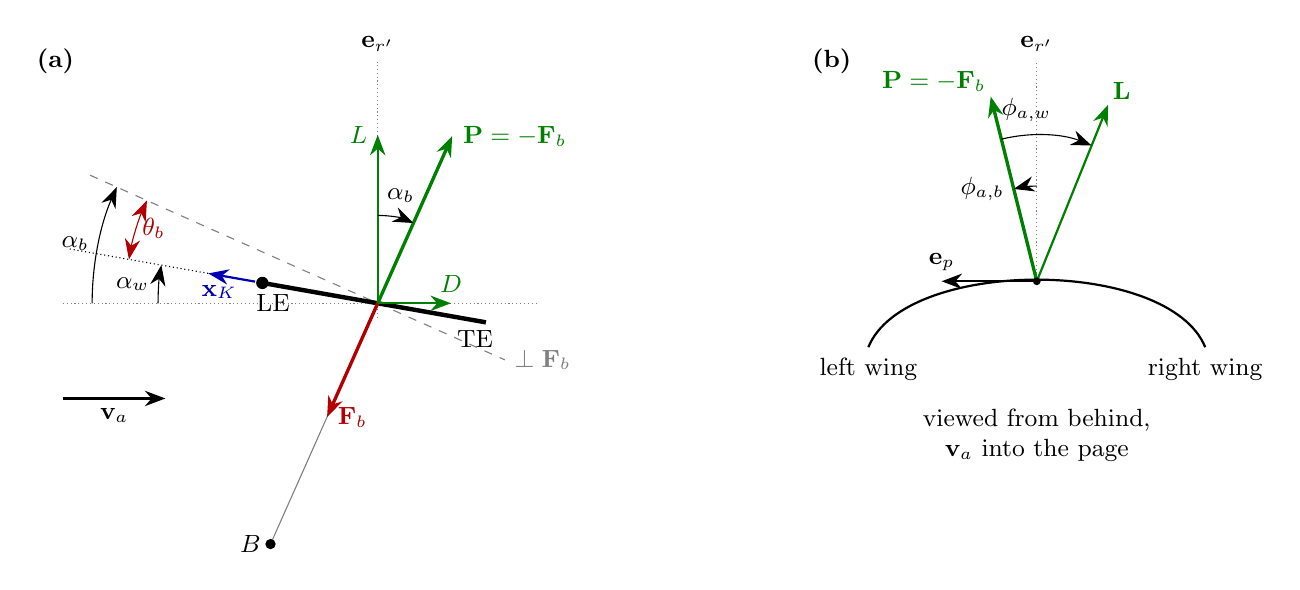
\begin{tikzpicture}[scale=0.93,>={Stealth[length=2.6mm]},
  lab/.style={font=\small},vec/.style={->,thick}]
  % ---------------- (a) side view ----------------
  \begin{scope}
    \def\aw{10}\def\ab{24}
    \coordinate (O) at (0,0);
    % references
    \draw[densely dotted,gray] (-4.3,0) -- (2.2,0);
    \draw[densely dotted,gray] (0,-0.2) -- (0,3.3) node[above,lab,black] {$\mathbf e_{r'}$};
    \draw[dashed,gray] (180-\ab:4.3) -- (-\ab:1.9);
    \node[lab,gray,anchor=west] at (-\ab:1.9) {$\perp\mathbf F_b$};
    % chord (centre panel)
    \draw[line width=1.6pt] (180-\aw:1.6) -- (-\aw:1.5);
    \fill (180-\aw:1.6) circle (2.4pt);
    \node[lab,anchor=north] at (180-\aw:1.45) {LE};
    \node[lab,anchor=north] at (-\aw:1.35) {TE};
    \draw[vec,blue!70!black] (180-\aw:1.7) -- (180-\aw:2.35);
    \node[lab,blue!70!black,anchor=north] at (180-\aw:2.2) {$\mathbf x_K$};
    \draw[densely dotted] (180-\aw:2.35) -- (180-\aw:4.3);
    % apparent wind
    \draw[vec] (-4.3,-1.3) -- (-2.9,-1.3) node[midway,below,lab] {$\mathbf v_a$};
    % lift, drag, wing pull
    \draw[vec,green!50!black] (O) -- (0,2.3) node[left,lab] {$L$};
    \draw[vec,green!50!black] (O) -- (1.0,0) node[above,lab] {$D$};
    \draw[vec,green!50!black,very thick] (O) -- (90-\ab:2.5)
      node[right,lab] {$\mathbf P=-\mathbf F_b$};
    % bridle and resultant
    \draw[gray] (O) -- (270-\ab:3.6) coordinate (B);
    \fill (B) circle (2pt) node[left,lab] {$B$};
    \draw[vec,red!70!black,very thick] (O) -- (270-\ab:1.7)
      node[right,lab] {$\mathbf F_b$};
    % angles, drawn on the upstream side beyond the chord
    \draw[->] (180:3.0) arc (180:180-\aw:3.0);
    \node[lab,anchor=east] at (180-\aw/2:3.0) {$\alpha_w$};
    \draw[->] (180:3.9) arc (180:180-\ab:3.9);
    \node[lab,anchor=east] at (180-\ab/2:3.9) {$\alpha_b$};
    \draw[<->,red!70!black] (180-\aw:3.45) arc (180-\aw:180-\ab:3.45);
    \node[lab,red!70!black,anchor=west] at (180-\aw/2-\ab/2:3.5) {$\theta_b$};
    \draw[->] (90:1.2) arc (90:90-\ab:1.2);
    \node[lab] at (90-\ab/2:1.5) {$\alpha_b$};
    \node[font=\bfseries\small] at (-4.4,3.3) {(a)};
  \end{scope}
  % ---------------- (b) view from behind ----------------
  \begin{scope}[xshift=9.0cm,yshift=0.3cm]
    \coordinate (O) at (0,0);
    \draw[thick] (-2.3,-0.9) .. controls (-1.8,0.33) and (1.8,0.33) .. (2.3,-0.9);
    \node[lab] at (-2.3,-1.2) {left wing};
    \node[lab] at (2.3,-1.2) {right wing};
    \draw[densely dotted,gray] (0,0) -- (0,3.0) node[above,lab,black] {$\mathbf e_{r'}$};
    \draw[vec] (O) -- (-1.3,0) node[above,lab] {$\mathbf e_p$};
    \draw[vec,green!50!black,very thick] (O) -- (90+14:2.6)
      node[above left=-2pt,lab] {$\mathbf P=-\mathbf F_b$};
    \draw[vec,green!50!black] (O) -- (90-22:2.6) node[above right=-2pt,lab] {$\mathbf L$};
    \draw[->] (90:1.3) arc (90:104:1.3);
    \node[lab,anchor=east] at (104:1.3) {$\phi_{a,b}$};
    \draw[->] (104:2.0) arc (104:68:2.0);
    \node[lab,anchor=south] at (94:2.05) {$\phi_{a,w}$};
    \fill (O) circle (1.5pt);
    \node[lab,align=center] at (0,-2.1) {viewed from behind,\\$\mathbf v_a$ into the page};
    \node[font=\bfseries\small] at (-2.8,3.0) {(b)};
  \end{scope}
\end{tikzpicture}
\caption{Geometric definitions (angles exaggerated). (a) Side view in the
wing's symmetry plane: centre-panel chord with axis $\mathbf x_K$, apparent
wind $\mathbf v_a$, the wing's lift and drag, the bridle resultant
$\mathbf F_b$ acting on the wing from the bridle point $B$ and its reverse
$\mathbf P$ (collinear with $\mathbf F_w$ for a massless kite). $\alpha_w$ is
the chord angle from the oncoming flow, $\alpha_b$ the angle of the line
perpendicular to $\mathbf F_b$ (equally, of $\mathbf P$ from
$\mathbf e_{r'}$), and $\theta_b=\alpha_b-\alpha_w$ the bridle pitch fixed
by the bridle geometry and depower setting. (b) Rear view about
$\mathbf v_a$: the bridle roll $\phi_{a,b}$ of $\mathbf P$ and the steering
roll $\phi_{a,w}$ of the lift relative to it, both measured positive toward
the left wing; drawn for $u_s>0$ (right turn, $\phi_{a,w}<0$).}
\label{fig:geometry}
\end{figure}

%======================================================================
\section{Simulation data required}
\label{sec:data}
Two kinds of simulation are needed, and the second is not optional.

\subsection{Converged trims}
\label{sec:data-trims}
A trim is a converged aerostructural equilibrium of the kite at a prescribed
wind and control setting: structure and aerodynamics coupled to convergence,
the forces and the moments about the bridle point balanced, the flight speed
(and for a steered trim the course rate) solved for. Conditions: centre of
the wind window, gravity off, the tether represented by its force at the
bridle point only.

\paragraph{Which trims.}
\begin{itemize}
  \item \textbf{Depower sweeps} at zero steering: the power tape across the
        whole band, at several apparent wind speeds
        ($v_a\approx13$--\SI{25}{\metre\per\second} here). They give
        $\theta_b(u_p)$ and the depower and load terms of the polars.
  \item \textbf{Steering sweeps} at the powered and the depowered setting,
        from zero to full steering (one side suffices; left and right are
        mirror images). They give $k_{\phi,s}$ and the steering terms.
\end{itemize}

\paragraph{What each trim must output.}
\begin{center}
\small
\begin{tabular}{lp{0.62\textwidth}}
\toprule
Quantity & Definition \\
\midrule
$u_p$, $u_s$ & controls of the trim \\
$\rho$, wind speed & air density, free-stream wind \\
$\mathbf v_a$ & apparent wind at the wing reference point (air relative to kite) \\
$\mathbf e_r$ & radial unit vector, ground station to kite \\
$\mathbf F_w$ & aerodynamic force on wing and bridle lines, without KCU \\
$\mathbf F_\mathrm{KCU}$ & KCU aerodynamic drag, separately \\
$\mathbf F_t$ & tether force at the bridle point \\
$m_w$, $m_\mathrm{KCU}$, $\mathbf a$ & wing and KCU mass, kite acceleration (or the inertial force), to build $\mathbf F_b$ \\
$P_\mathrm{LE}$, $P_\mathrm{TE}$, $\mathbf s$ & centre-panel chord points and span direction of the \emph{deformed} wing \\
$v_\tau$, $\dot\chi$ & trimmed tangential speed and course rate \\
deformed shape & the full converged structural geometry, to be frozen for the sweeps of Sect.~\ref{sec:data-sweeps} \\
convergence & flag and force/moment residuals \\
\bottomrule
\end{tabular}
\end{center}
From these, Sect.~\ref{sec:geometry} gives per trim $\alpha_w$, $C_L$,
$C_D$, $\alpha_b$, $\theta_b$, $\phi_{a,b}$ and $\phi_{a,w}$.

\subsection{Angle-of-attack sweeps on the frozen shapes}
\label{sec:data-sweeps}
Trims alone cannot identify the polars. Along a trimmed depower sweep
$\alpha_w$ follows $u_p$ almost one to one (it moves by about
\SI{1}{\degree} across the whole $v_a$ range), so a fit on trims cannot tell
the polar slope from the depower effect. In flight, gravity and turning move
$\alpha_w$ by several degrees around the trim value, and the ROM needs the
polar there. Around every trim:
\begin{enumerate}
  \item freeze the converged deformed shape (no further structural solve);
  \item keep $|\mathbf v_a|$, the sideslip and the body rates of the trim, and
        rotate the inflow about $\mathbf y_K$ in steps of $\Delta\alpha_w$, here
        from \SI{-6}{\degree} to \SI{+22}{\degree} about the trim, through
        the stall;
  \item solve the aerodynamics only at each step, without re-trimming (the
        moment about the bridle point is not balanced; this is the polar of
        that shape);
  \item record per step $\alpha_w$ (Eq.~\ref{eq:alpha-w}), $\mathbf v_a$,
        $\mathbf F_w$ and, separately, $\mathbf F_\mathrm{KCU}$.
\end{enumerate}
The $\Delta\alpha_w=0$ step must reproduce the trim's $C_L$ (here within
\lensTolPct\,\%); a sweep that does not is discarded and its trim enters as a
single sample (the lens check below).

\subsection{The LEI-V3 data set}

\paragraph{Coupled trims (anchors).}
\nAnchorsAll{} converged coupled VSM + Billow-wireframe trims (VSM main at
\code{8825a12}, artificial viscosity on, 45 panels) from the \code{\_billow9}
continuation chains of the 2019 hardware: power-tape sweeps at zero steering
for $v_a=13$--\SI{25}{\metre\per\second}, and steering sweeps at the reel-out
and reel-in depower.

\paragraph{Frozen-shape polars.}
Each anchor's snapshot is frozen, re-trimmed with the aerodynamics alone as
a consistency check, and swept as above
(\code{run\_center\_sweep\_alpha\_polar.py}).

\paragraph{Lens check.}
A polar is used only if its frozen-shape re-trim reproduces the coupled trim:
$C_L$ at the coupled $\alpha$ within \lensTolPct\,\%. Steered snapshots with a
steering tape of \SI{0.125}{\metre} or more re-trim to a different roll/rate
state ($\alpha$ up to \SI{2}{\degree} off, $C_L$ 10--23\,\% high); their polars
are dropped and their coupled trims enter as single samples instead.

\paragraph{Sample.}
Within the depower band and up to $\alpha=\SI{30}{\degree}$:
\nPolarSamples{} polar samples and \nTrimSamples{} coupled-trim samples from
\nAnchorsFit{} anchors.

%======================================================================
\section{Identification method}
\label{sec:method}

\begin{center}
\small
\begin{tabular}{lll}
\toprule
Parameter & Data & Fit \\
\midrule
$\theta_0$, $\theta_1$ & unsteered trims & $\theta_b=\alpha_b-\alpha_w$, linear in $u_p$ \\
$k_{\phi,s}$ & steered trims & $\phi_{a,w}$, linear in $u_s$ through the origin \\
$\alpha_s$, $w$ & sweeps + trims & grid search on the $C_L$ cross-validation error \\
$C_L$, $C_D$ terms & sweeps + trims & stepwise least squares in $(\alpha_w,u_p,u_s,v_a,\sigma)$ \\
\bottomrule
\end{tabular}
\end{center}
LEI-V3 values for comparison: $\theta_b=\SI{\thetaPoweredDeg}{\degree}$ at
$u_p=\SI{1.7}{\metre}$ and \SI{\thetaDepoweredDeg}{\degree} at
\SI{2.1}{\metre}; $k_{\phi,s}=\rollGain$\,rad.
\subsection{Bridle pitch}
With gravity off, the coupled equilibrium is
$\mathbf F_\mathrm{wing}+\mathbf F_\mathrm{KCU}+\mathbf F_t+\mathbf F_\mathrm{in}=0$,
and the ROM's bridle resultant is
$\mathbf F_b=-(\mathbf F_\mathrm{wing}+\tfrac{m_w}{m}\mathbf F_\mathrm{in})$.
$\alpha_b$ is its paper Eq.~D11 angle about the apparent wind and $\alpha_w$ the
centre-panel angle; $\theta_b=\alpha_b-\alpha_w$ is fitted linearly in $u_p$ by
ordinary least squares on the \thetaN{} unsteered trims in the band.

\subsection{Steering gain}
$\phi_{a,w}$ is the roll of the wing lift about $\mathbf v_a$ relative to
$-\mathbf F_b$ (paper Eqs.~D6--D8, D13); $k_{\phi,s}$ is the least-squares slope
through the origin over the \rollN{} steered trims.

\subsection{Stall location}
$\alpha_s$ and $w$ are chosen first, on a grid
($\alpha_s=15.5$--\SI{18}{\degree}, $w=0.5$--\SI{1.5}{\degree}), by the
cross-validation error of the full $C_L$ library with fixed terms. This
separates locating the stall from choosing the terms.

\subsection{Candidate terms}
\begin{center}
\begin{tabular}{lll}
\toprule
Group & Terms & Reason \\
\midrule
attached polar & $\alpha$, $\alpha^2$ & lift slope and curvature \\
depower & $u_p$, $u_p^2$, $\alpha u_p$, $\alpha^2u_p$ & shape change with the power tape \\
steering & $u_s^2$, $\alpha u_s^2$, $u_pu_s^2$ & symmetric in left/right steering \\
load & $v_a$, $\alpha v_a$, $u_pv_a$ & deformation grows with dynamic pressure \\
stall & $\sigma$, $\sigma\alpha$, $\sigma\alpha^2$, $\sigma u_p$, $\sigma u_s^2$ & active past the stall only \\
\bottomrule
\end{tabular}
\end{center}
There is no $\alpha^3$: the ROM's solvers do not bound $\alpha$, a cubic $C_D$
went negative beyond the data, and a cubic $C_L$ cannot follow the sharp stall.

\subsection{Least squares and selection}
For a term set $\mathcal T$, the coefficients minimise the sum of squared
residuals, $\hat{\mathbf c}=\arg\min_{\mathbf c}\lVert\mathbf y-X_\mathcal T\mathbf c\rVert_2^2$,
solved with each column scaled to unit RMS for conditioning and mapped back.

Polar samples of one frozen shape are strongly correlated, so the selection
score is the \emph{grouped} $K$-fold cross-validation error with whole anchors
held out ($K=5$):
\begin{equation}
  \mathrm{CV}(\mathcal T)=\frac1K\sum_{k=1}^K
  \sqrt{\frac{1}{|G_k|}\sum_{i\in G_k}\bigl(y_i-\hat y_i^{(-k)}\bigr)^2},
\end{equation}
where $\hat y^{(-k)}$ is fitted without fold $G_k$. A random split would score
interpolation inside a polar rather than prediction at an unseen state. BIC
is not used: it treats the correlated samples as independent evidence and
keeps accepting terms worth a fraction of a percent.

\begin{enumerate}
  \item \textbf{Forward}: from the intercept, add the candidate that lowers
        $\mathrm{CV}$ most; stop when the best improves it by less than
        \minImprovementPct\,\%.
  \item \textbf{Backward}: drop any term whose removal costs less than the same
        \minImprovementPct\,\%; a term picked early can become redundant later.
  \item \textbf{Extrapolation check}: $C_D$ must stay positive over
        $\pm\SI{30}{\degree}$ across the fitted $u_p$, $u_s$, $v_a$ ranges, or
        the identification fails.
\end{enumerate}

\subsection{Metrics and uncertainty}
Reported are the in-sample RMSE and $R^2=1-\sum r_i^2/\sum(y_i-\bar y)^2$ per
$\alpha$ band, and the grouped CV RMSE.

The coefficient intervals are an \emph{anchor-cluster bootstrap}: \nBoot{}
resamples draw anchors with replacement, refit the selected terms on their
samples, and report the 2.5/97.5\,\% percentiles. Resampling whole anchors
respects the within-shape correlation that makes ordinary least-squares
standard errors far too optimistic. The intervals are \emph{conditional on the
selected term set}: the selection is not repeated per resample. $\theta_b$
and $k_{\phi,s}$ have one sample per trim, and their standard errors are the
ordinary least-squares ones.

%======================================================================
\section{Results}
\label{sec:results}

\subsection{Identified coefficients}
\begin{table}[H]
\centering\small
\caption{Selected $C_L$ and $C_D$ terms ($\alpha$ in rad, $u_p$ in m, $v_a$ in
\si{\metre\per\second}) with anchor-cluster bootstrap 95\,\% intervals.}
\begin{tabular}{llrrr}
\toprule
Coefficient & Term & Estimate & \multicolumn{2}{c}{95\,\% interval} \\
\midrule
$C_L$ & $1$ & $0.3838$ & $0.3593$ & $0.4074$ \\
 & $\alpha\,u_p$ & $-0.625$ & $-0.7445$ & $-0.5141$ \\
 & $\alpha^{2}\,\sigma$ & $5.406$ & $4.585$ & $6.309$ \\
 & $\alpha$ & $5.459$ & $5.249$ & $5.68$ \\
 & $\alpha^{2}$ & $-6.898$ & $-7.391$ & $-6.4$ \\
 & $\alpha\,\sigma$ & $-6.061$ & $-6.791$ & $-5.381$ \\
 & $\alpha\,u_s^{2}$ & $-39.74$ & $-44.01$ & $-34.93$ \\
 & $u_s^{2}\,\sigma$ & $14.2$ & $12.16$ & $16$ \\
 & $u_p$ & $-0.04595$ & $-0.05984$ & $-0.03291$ \\
 & $v_a$ & $0.0009956$ & $0.0007995$ & $0.001174$ \\
 & $\sigma$ & $0.9579$ & $0.8246$ & $1.101$ \\
 & $\alpha^{2}\,u_p$ & $1.82$ & $1.581$ & $2.057$ \\
\midrule
$C_D$ & $1$ & $0.0818$ & $0.08147$ & $0.08216$ \\
 & $\alpha^{2}$ & $1.277$ & $1.256$ & $1.297$ \\
 & $\alpha$ & $0.1191$ & $0.1109$ & $0.1285$ \\
 & $\alpha^{2}\,\sigma$ & $-0.8711$ & $-0.964$ & $-0.7737$ \\
 & $u_p\,\sigma$ & $-0.02216$ & $-0.02959$ & $-0.01426$ \\
 & $\alpha\,v_a$ & $0.001259$ & $0.000725$ & $0.001685$ \\
 & $\alpha\,\sigma$ & $0.4555$ & $0.3783$ & $0.5291$ \\
 & $u_s^{2}$ & $-0.5255$ & $-0.6016$ & $-0.4706$ \\
 & $\alpha\,u_s^{2}$ & $2.474$ & $1.535$ & $3.861$ \\
\bottomrule
\end{tabular}

\end{table}

\begin{table}[H]
\centering\small
\caption{Selection path: the term added ($+$) or removed ($-$) at each step and
the grouped CV RMSE after it.}
\begin{tabular}{rlr@{\hspace{2.5em}}rlr}
\toprule
\multicolumn{3}{c}{$C_L$} & \multicolumn{3}{c}{$C_D$} \\
Step & Term & CV RMSE & Step & Term & CV RMSE \\
\midrule
0 & intercept & $0.31$ & 0 & intercept & $0.0977$ \\
1 & $+\alpha\,u_p$ & $0.196$ & 1 & $+\alpha^2$ & $0.0106$ \\
2 & $+\alpha^2\,\sigma$ & $0.0814$ & 2 & $+\alpha$ & $0.00664$ \\
3 & $+\alpha$ & $0.0362$ & 3 & $+\sigma$ & $0.00572$ \\
4 & $+\alpha^2$ & $0.0282$ & 4 & $+\alpha^2\,\sigma$ & $0.00521$ \\
5 & $+\alpha\,\sigma$ & $0.0243$ & 5 & $+\sigma\,u_p$ & $0.00499$ \\
6 & $+\alpha\,u_s^2$ & $0.0233$ & 6 & $+\alpha\,v_a$ & $0.00484$ \\
7 & $+\sigma\,u_s^2$ & $0.0226$ & 7 & $+\alpha\,\sigma$ & $0.00472$ \\
8 & $+\sigma\,u_p$ & $0.0216$ & 8 & $+u_s^2$ & $0.00465$ \\
9 & $+u_p$ & $0.0212$ & 9 & $+\alpha\,u_s^2$ & $0.00459$ \\
10 & $+v_a$ & $0.0207$ & 10 & $-\sigma$ & $0.00462$ \\
11 & $+\sigma$ & $0.0205$ &  &  &  \\
12 & $+\alpha^2\,u_p$ & $0.0202$ &  &  &  \\
13 & $-\sigma\,u_p$ & $0.0202$ &  &  &  \\
\bottomrule
\end{tabular}

\end{table}

\begin{table}[H]
\centering\small
\caption{Fit quality per angle-of-attack band (all fitted samples).}
\begin{tabular}{lrrrr}
\toprule
Samples & $n$ & RMSE $C_L$ & RMSE $C_D$ & $R^2$ ($C_L$ / $C_D$) \\
\midrule
all & 4882 & $0.0201$ & $0.00458$ & 0.9958 / 0.9978 \\
$\alpha<13^\circ$ (operating) & 2915 & $0.0125$ & $0.00307$ & 0.9983 / 0.9906 \\
$13^\circ\le\alpha<19^\circ$ (stall) & 960 & $0.0381$ & $0.00759$ & 0.8212 / 0.9457 \\
$\alpha\ge19^\circ$ (post-stall) & 1007 & $0.0112$ & $0.00441$ & 0.7349 / 0.9818 \\
\midrule
\multicolumn{2}{l}{Grouped 5-fold CV RMSE} & $0.0202$ & $0.00462$ & \\
\bottomrule
\end{tabular}

\end{table}

\paragraph{Stall.} $\alpha_s=\SI{\stallDeg}{\degree}$, $w=\SI{\stallWidthDeg}{\degree}$.
Every coupled polar peaks near $C_L\approx1.2$ at 15.5--\SI{16.7}{\degree} and
drops within about \SI{2}{\degree} to a plateau near $0.87$. The stall band
carries the largest residual, because one polynomial family has to follow a
sharp drop; the operating range below \SI{13}{\degree} is fitted to a $C_L$ RMSE
of about $0.012$.

\paragraph{Bridle pitch.}
$\theta_0=\thetaZero\pm\thetaZeroSE$\,rad and
$\theta_1=\thetaSlope\pm\thetaSlopeSE$\,rad\,m$^{-1}$ (residual
\SI{\thetaRMSdeg}{\degree} RMS): $\theta_b=\SI{\thetaPoweredDeg}{\degree}$ at
\SI{1.7}{\metre} and \SI{\thetaDepoweredDeg}{\degree} at \SI{2.1}{\metre}.
The semi-empirical ROM measured its pitch against the tether direction instead
(KCU drag inside its $C_D$); that angle reads about \SI{2.5}{\degree} larger on
the same trims (Fig.~\ref{fig:theta}) and is not the $\theta_b$ defined here.
Its slope is 45\,\% steeper.

\paragraph{Steering gain.}
$k_{\phi,s}=\rollGain\pm\rollGainSE$\,rad per unit $u_s$ (residual
\SI{\rollRMSdeg}{\degree} RMS), against $-0.689$ for the semi-empirical ROM in
the same units.

\begin{figure}[H]
\centering
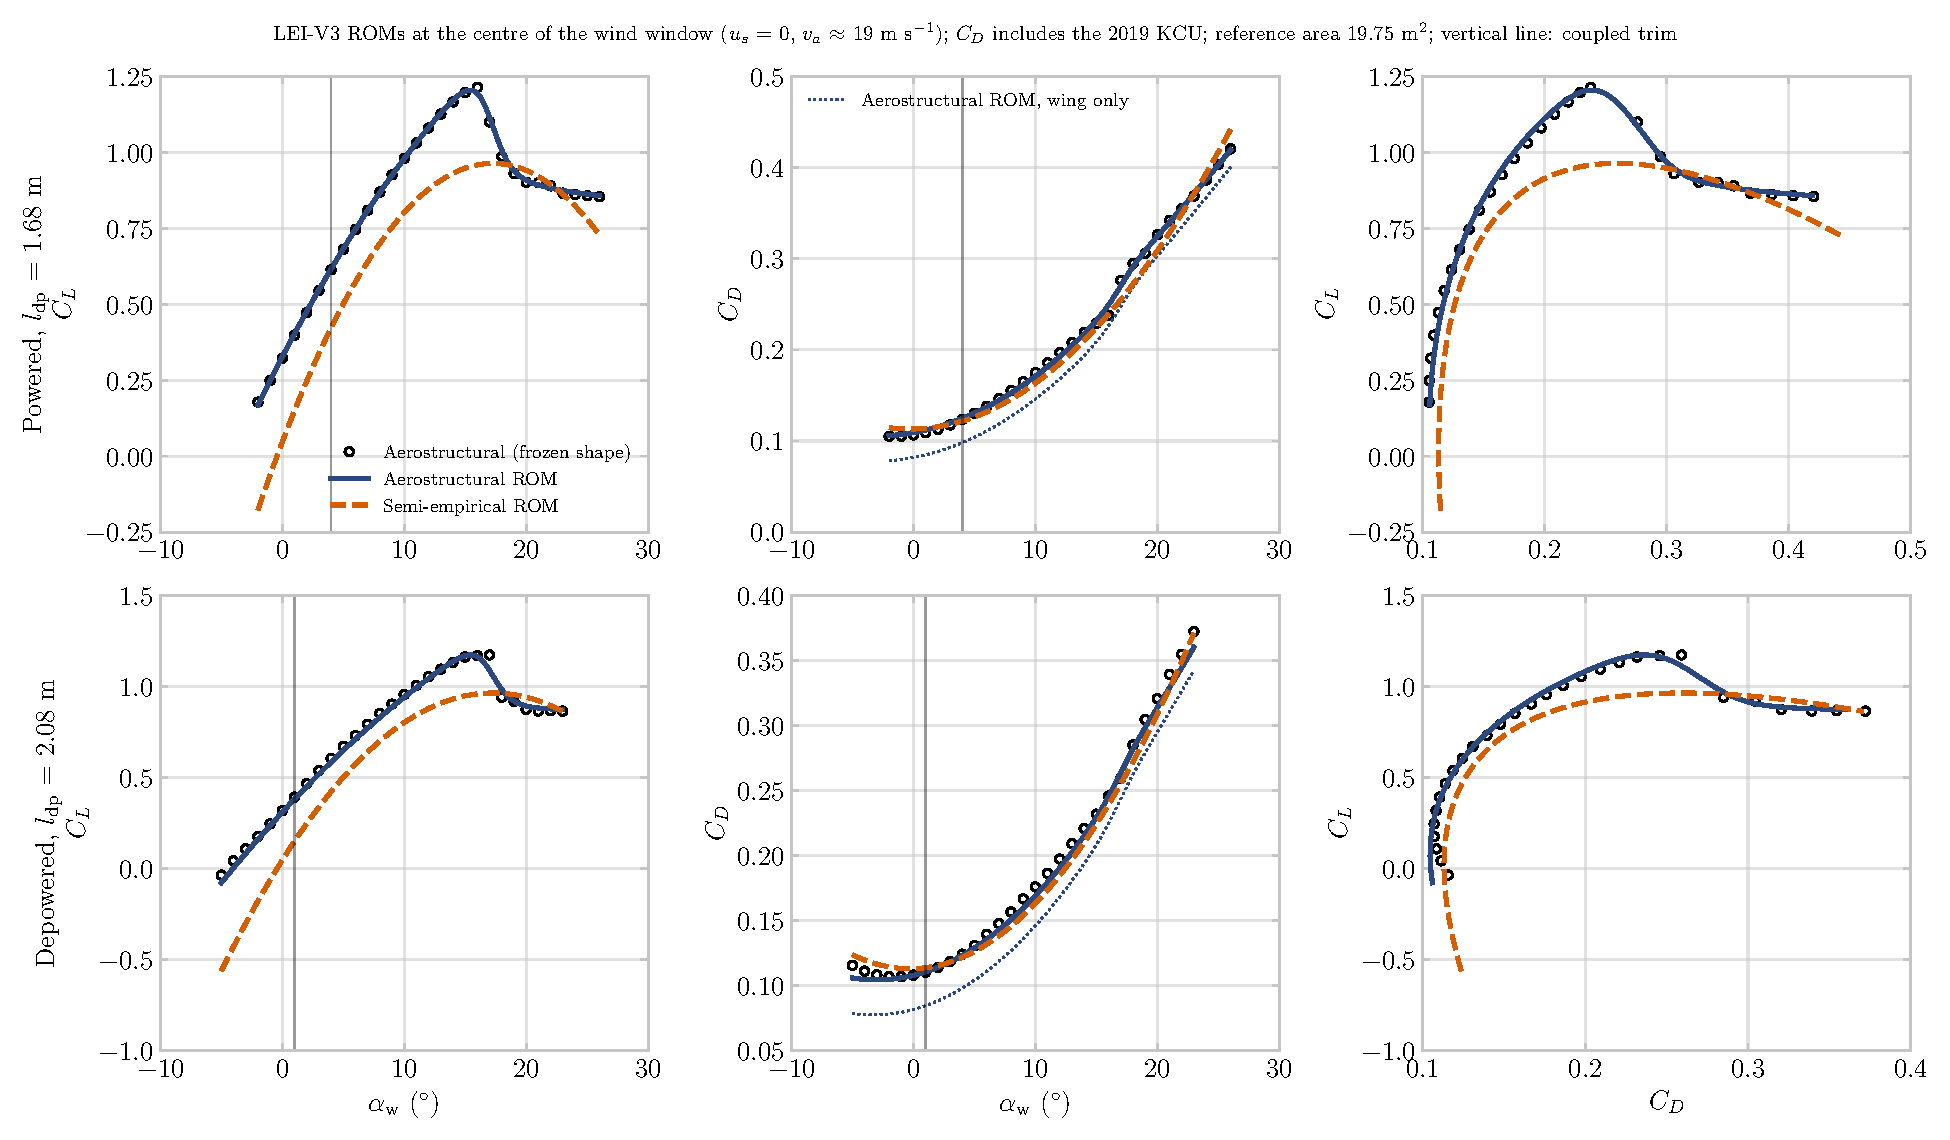
\includegraphics[width=\textwidth]{polars.pdf}
\caption{Lift and drag polars at the powered and depowered setting
($u_s=0$, $v_a\approx\SI{19}{\metre\per\second}$, $C_D$ with the 2019 KCU): coupled
frozen-shape data, the aerostructural ROM and the semi-empirical ROM.}
\label{fig:polars}
\end{figure}

\begin{figure}[H]
\centering
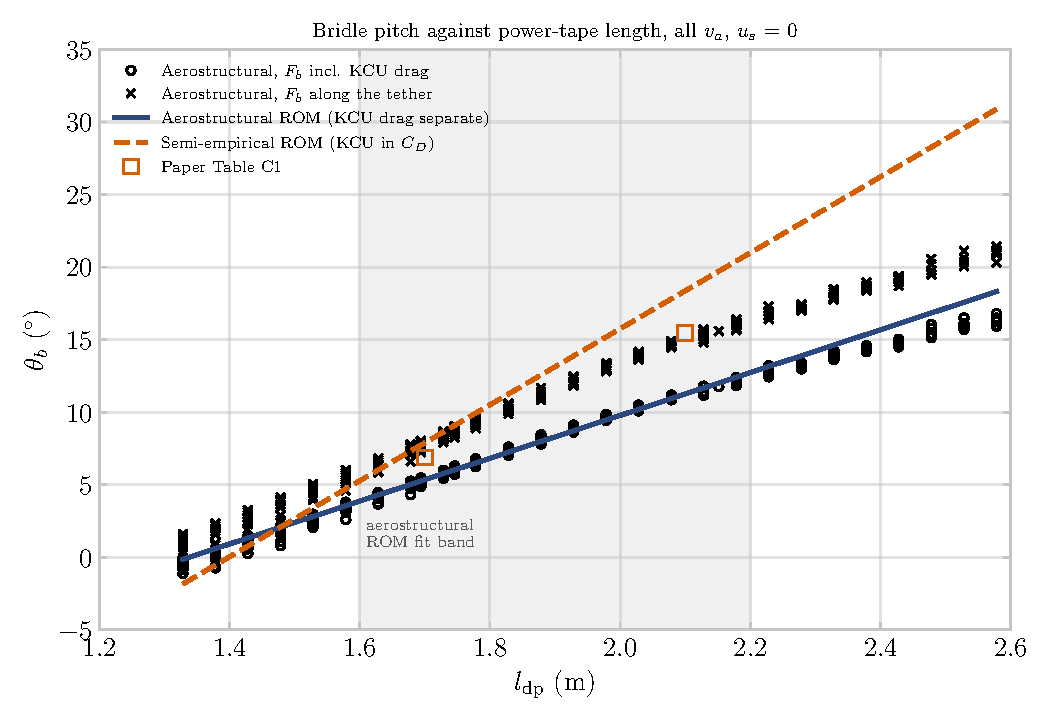
\includegraphics[width=0.75\textwidth]{theta_b.pdf}
\caption{Bridle pitch against power-tape length: coupled trims measured
against the bridle resultant ($\theta_b$) and against the tether direction,
the aerostructural relation and the semi-empirical one.}
\label{fig:theta}
\end{figure}

\subsection{Check against the coupled trims}
Each coupled trim is re-solved with the ROM's own quasi-steady solver at the
same condition: centre of the window, same wind, $u_p$, $u_s$, gravity off,
tetherless (\code{validate\_rom\_aerostructural.py}).

\begin{table}[H]
\centering\small
\caption{ROM against the coupled trims it was identified from: mean $\pm$
standard deviation of the relative errors.}
\begin{tabular}{llrrrr}
\toprule
ROM & Trims & $n$ & $v_\tau$ error (\%) & $F_t$ error (\%) & $\alpha_w$ error (\si{\degree}) \\
\midrule
Aerostructural & unsteered & 99 & $+0.1\pm1.5$ & $+2.9\pm6.2$ & $+0.07\pm0.16$ \\
 & steered & 144 & $-0.9\pm1.3$ & $+0.1\pm4.3$ & $+0.24\pm0.21$ \\
\midrule
Semi-empirical & unsteered & 99 & $-18.9\pm4.8$ & $-38.9\pm8.7$ & $+1.64\pm0.16$ \\
 & steered & 144 & $-15.3\pm2.4$ & $-26.1\pm8.2$ & $+2.06\pm0.24$ \\
\bottomrule
\end{tabular}

\end{table}

\subsection{Flight validation}
The 2019 flight (cycles 60--67) is reconstructed sample by sample with the
quasi-steady ROM on the flown hardware, in two modes:
\begin{itemize}
  \item \textbf{$\dot\chi$ in}: the measured turn rate is prescribed and the ROM
        solves the steering it needs, as in the paper's Fig.~8.
  \item \textbf{$u_s$ in}: the logged steering, plus the 2019 rig's zero offset
        ($-0.01645/1.4$), is fed in and the ROM solves the turn rate. This is
        the paper's causality, with $u_s$ an input and $\dot\chi$ algebraic.
\end{itemize}
The $\dot\chi$-in mode is also run with the discretised Williams tether (10
inelastic elements, sag and per-element drag; \code{--tether williams}),
solved together with the ground closure for the tether length and the angles
of its last element. The optimisations keep the rigid tether; the Williams
rows test whether the reconstruction errors come from it.

Every number in this section is on the corrected bridle-angle frame of
Sect.~\ref{sec:frame}. The first validation runs, on the frame the ROM code
had used since the paper, read very differently (aerostructural reel-out
$+49\,\%$ tension, semi-empirical $+11\,\%$) and led the flight correction of
Sect.~\ref{sec:flight-correction} astray for a day; they are kept under
\path{results/LEI-V3-KITE/rom_validation_oldframe/} for the record only.

The quasi-steady equations have a pre-stall root and a spurious post-stall one.
A root at or past the ROM's stall angle is retried from faster speed guesses,
and kept and flagged if no pre-stall root turns up. Every converged root is
scored, and the pre-stall share is reported. The speed stability
$\partial\dot v_\tau/\partial v_\tau$ at fixed controls (paper Eq.~36) is
reported as a diagnostic only: it selects correctly in crosswind flight, but
every flown reel-in state reads as unstable (Sect.~\ref{sec:open}).

\IfFileExists{generated/flight.tex}{%
\begin{table}[H]
\centering\scriptsize
\caption{Flight validation, 2019 cycles 60--67: medians of the relative errors
(tension interquartile range in brackets) and of the absolute turn-rate error,
over the samples that converged (Solved). In the $\dot\chi$-in mode the
solved steering is regressed on the logged steering plus the zero offset
(slope and correlation; medians of $|u_s|$ are not a valid check, thousands
of near-zero samples make them read $2\times$ for a slope of one).}
\label{tab:flight}
\resizebox{\textwidth}{!}{\begin{tabular}{llllrrrrrrr}
\toprule
Tether & Mode & ROM & Phase & Solved (\%) & Pre-stall (\%) & Speed-stable (\%) & $F_t$ error (\%) & $v_\tau$ error (\%) & $u_s$ slope (corr) & $|\Delta\dot\chi|$ (\si{\radian\per\second}) \\
\midrule
rigid & $\dot\chi$ in & semi-empirical & reel-out & 90 & 100.0 & 96.9 & $-10.1$ (-34..+22) & $-6.28$ & 0.95 (0.91) & -- \\
 &  & semi-empirical & reel-in & 88 & 100.0 & 0.3 & $-6.48$ (-28..+17) & $-17.8$ & 0.90 (0.66) & -- \\
 &  & aerostructural & reel-out & 89 & 99.8 & 89.1 & $7.43$ (-24..+43) & $9.64$ & 1.58 (0.90) & -- \\
 &  & aerostructural & reel-in & 100 & 100.0 & 0.0 & $102$ (+66..+138) & $72.2$ & 1.21 (0.61) & -- \\
 &  & aerostructural-flight & reel-out & 91 & 99.6 & 65.5 & $-2.92$ (-29..+30) & $-0.606$ & 0.88 (0.89) & -- \\
 &  & aerostructural-flight & reel-in & 98 & 100.0 & 0.0 & $32.3$ (+6..+59) & $0.426$ & 0.89 (0.65) & -- \\
\midrule
rigid & $u_s$ in & semi-empirical & reel-out & 93 & 100.0 & 99.0 & $-5.65$ (-30..+25) & $-1.09$ & -- & $0.29$ \\
 &  & semi-empirical & reel-in & 88 & 100.0 & 0.6 & $-4.56$ (-27..+22) & $-17$ & -- & $0.13$ \\
 &  & aerostructural & reel-out & 97 & 100.0 & 97.4 & $23.1$ (-5..+53) & $14.2$ & -- & $0.26$ \\
 &  & aerostructural & reel-in & 100 & 100.0 & 0.0 & $102$ (+67..+138) & $73$ & -- & $0.092$ \\
 &  & aerostructural-flight & reel-out & 94 & 100.0 & 96.1 & $1.33$ (-24..+31) & $3.57$ & -- & $0.27$ \\
 &  & aerostructural-flight & reel-in & 99 & 100.0 & 0.0 & $33.3$ (+6..+61) & $0.859$ & -- & $0.14$ \\
\midrule
Williams & $\dot\chi$ in & semi-empirical & reel-out & 90 & 99.6 & 95.9 & $-9.03$ (-35..+25) & $-4.51$ & 0.94 (0.92) & -- \\
 &  & semi-empirical & reel-in & 72 & 100.0 & 1.2 & $-18.4$ (-36..+6) & $-26.5$ & 1.10 (0.66) & -- \\
 &  & aerostructural & reel-out & 88 & 99.0 & 90.7 & $13.7$ (-21..+52) & $12$ & 1.58 (0.90) & -- \\
 &  & aerostructural & reel-in & 99 & 100.0 & 0.0 & $88.2$ (+50..+123) & $65.8$ & 1.24 (0.60) & -- \\
 &  & aerostructural-flight & reel-out & 88 & 98.7 & 71.8 & $-0.172$ (-29..+36) & $2.39$ & 0.89 (0.91) & -- \\
 &  & aerostructural-flight & reel-in & 94 & 100.0 & 0.0 & $20$ (-7..+45) & $-6.7$ & 0.93 (0.63) & -- \\
\bottomrule
\end{tabular}
}
\end{table}}{\textit{(flight tables not generated yet)}}

\IfFileExists{figures/flight_solved.pdf}{%
\begin{figure}[H]
\centering
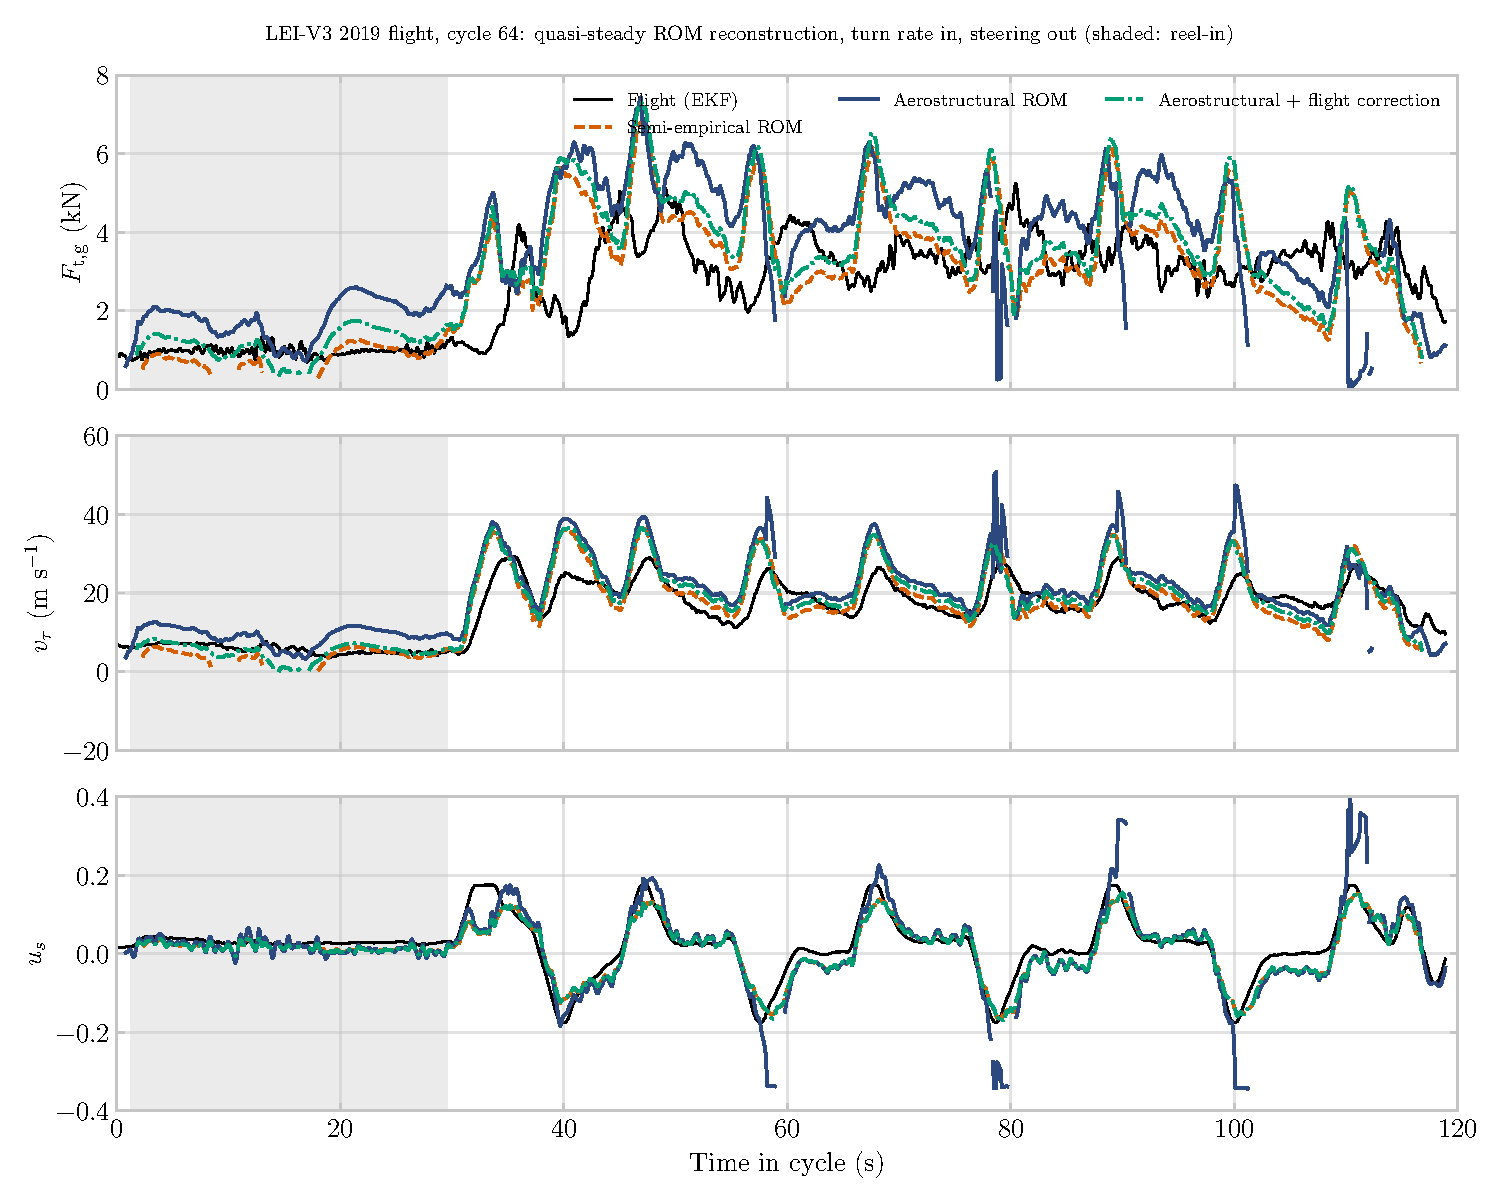
\includegraphics[width=\textwidth]{flight_solved.pdf}
\caption{Cycle 64 (held out) with the measured turn rate as input and the
steering solved: ground tension, tangential speed and the steering each ROM
needs, against the EKF reconstruction (solid black, logged $u_s$ with the
rig's zero offset). Shaded: reel-in. Gaps are samples without a converged
root.}
\label{fig:flight-solved-64}
\end{figure}}{}

\IfFileExists{figures/flight_solved_cycle61.pdf}{%
\begin{figure}[H]
\centering
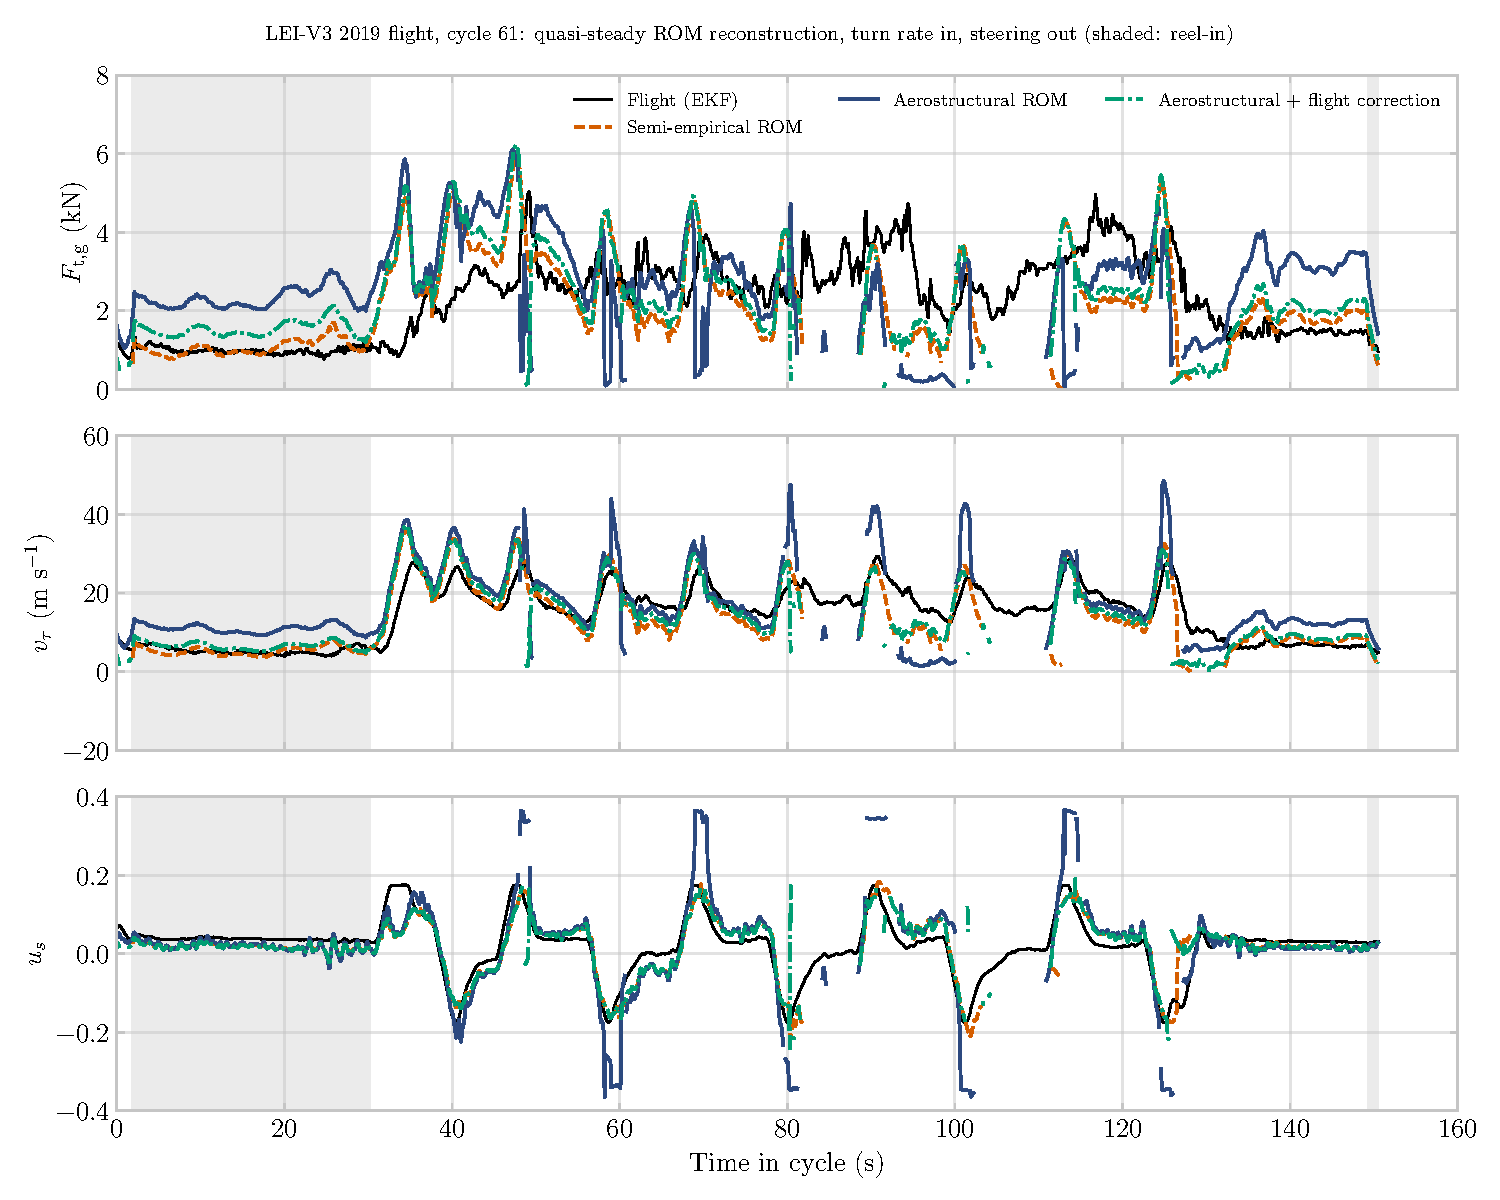
\includegraphics[width=\textwidth]{flight_solved_cycle61.pdf}
\caption{As Fig.~\ref{fig:flight-solved-64} for cycle 61.}
\label{fig:flight-solved-61}
\end{figure}}{}

\IfFileExists{figures/flight_measured.pdf}{%
\begin{figure}[H]
\centering
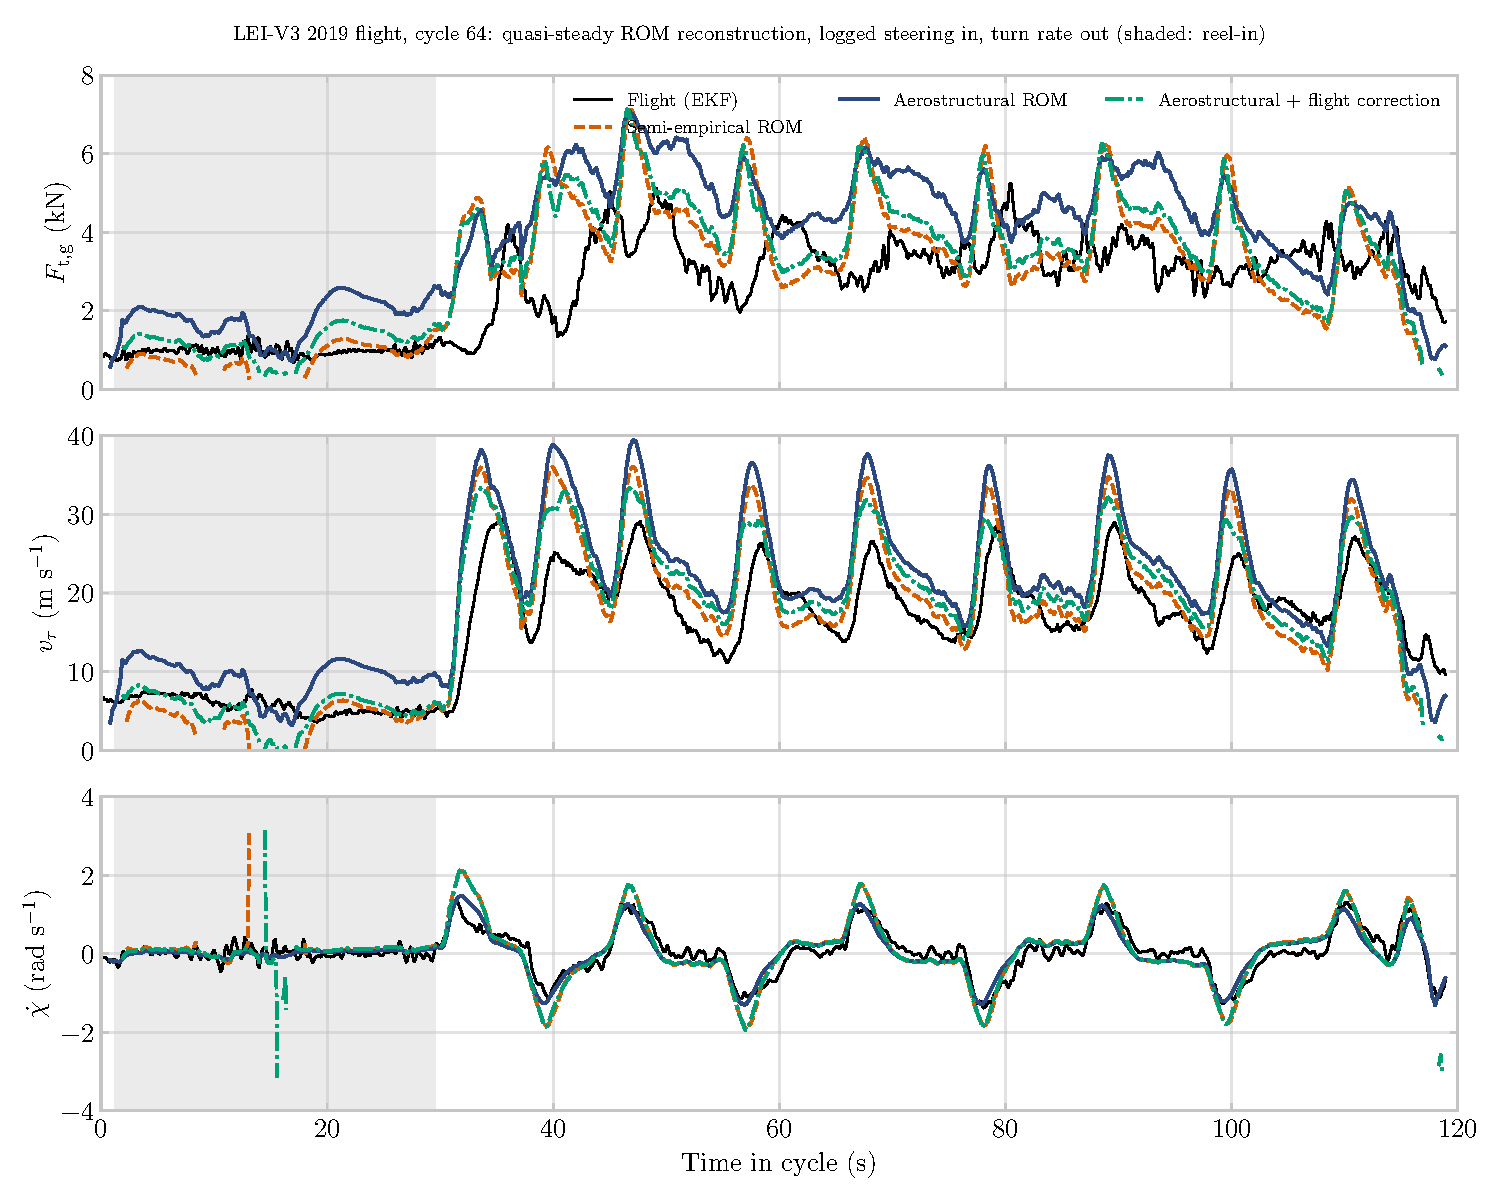
\includegraphics[width=\textwidth]{flight_measured.pdf}
\caption{Cycle 64 with the logged steering as input.}
\end{figure}}{}

With the measured turn rate as input, the simulation-only ROM reproduces the
held-out reel-out to $+7\,\%$ in tension and $+10\,\%$ in speed, with no
flight data in it at all; with the logged steering as input, to $+23\,\%$ and
$+14\,\%$. It still flies somewhat faster than the kite did, which is the
direction of the VSM's known drag deficit~\cite{poland2025wind}, but the
deficit is a fraction of what the uncorrected frame had made it look like.
Its solved steering has slope 1.6 against the logged steering: the
aerostructural roll gain ($-0.53$) is too weak, by exactly that factor
(Sect.~\ref{sec:flight-correction}). The semi-empirical rows are the paper's
ROM \emph{recalibrated} on the corrected frame with the step-3 method of
Sect.~\ref{sec:flight-correction} ($\theta_b$, $C_{D,0}$, the $|u_s|$ drag
and the roll gain; \code{refine\_rom\_flight\_output\_error.py --rom
semi\_empirical}, the paper's values kept in the file's comments): reel-out
$-10\,\%$/$-6\,\%$ with the turn rate in and $-6\,\%$/$-1\,\%$ with the
logged steering in, its reel-in tension within $-6\,\%$ but its reel-in
speed $-18\,\%$. Its recalibrated gain, $-0.69$, is the paper's. After this
comparison the semi-empirical ROM was removed from the repository (archived
in git history; \code{config\_paths} keeps its path): the flight-corrected
aerostructural ROM is the better-founded model and is now the default in
every LEI-V3 system file. The rows and figures here are kept as the record.

Reel-in is where the aerostructural polar fails: that ROM doubles the
tension, and the flight-corrected one (aerostructural-flight rows,
Sect.~\ref{sec:flight-correction}), which brings the reel-out within a few
percent in both modes, still reads $+33\,\%$ there. The recalibrated
semi-empirical ROM does better on reel-in tension but not on reel-in speed;
Sect.~\ref{sec:open} discusses why reel-in resists.

The tether model is not what separates the ROMs. With the Williams tether
the reel-out errors move by a few points (aerostructural $+14\,\%$/$+12\,\%$,
flight-corrected $+6\,\%$/$+4\,\%$, semi-empirical $-20\,\%$/$-11\,\%$) and
the steering regressions are unchanged. On reel-in it helps the
flight-corrected ROM ($+33\to+21\,\%$ tension) and costs the semi-empirical
one most of its roots (\SI{34}{\percent} solved).

%======================================================================
\section{The bridle-angle frame}
\label{sec:frame}
The ROM takes two angles of the bridle resultant $\mathbf F_b$ about the
apparent wind: the bridle pitch $\alpha_b$ (paper Eq.~D11), from which
$\alpha_w=\alpha_b-\theta_b$, and the bridle roll $\phi_b$ (Eqs.~D6--D8), the
reference the steering roll $k_{\phi,s}u_s$ is measured from. In
\code{awetrim.system.kite} both were computed by rotating $\mathbf F_b$ into
an Euler-angle ``aerodynamic'' frame built from the pitch and yaw of
$\mathbf v_a$. Checked numerically on a flown state with sideslip (the
apparent wind having a component normal to the course), that frame's $x$ axis
was not along $\mathbf v_a$: $\hat{\mathbf x}_A\cdot\hat{\mathbf v}_a=-0.97$,
and flipping the sign of the yaw angle gives $-1.0000$ exactly. The yaw sign
was mirrored for the rotation order used, so the frame sat at twice the
sideslip angle off $\mathbf v_a$ in the tangent plane, with the normal axis
off by the same amount. The lift direction, built directly from the
$\mathbf v_a$ vector elsewhere in the same class, was right.

The error is zero at zero sideslip: the centre-window trims the
aerostructural ROM was identified on and checked against
(Sect.~\ref{sec:results}) have none. In crosswind flight the apparent wind
has a normal component of 3--\SI{5}{\metre\per\second} at
\SI{20}{\metre\per\second}, a sideslip of 7--14$^\circ$, and the frame error
let the normal component of $\mathbf F_b$ --- the KCU's inertia in a turn,
some \SI{600}{\newton} on \SI{5}{\kilo\newton} --- leak into the pitch and
the roll. On cycle 64 the bridle pitch came out 2.3--3.0$^\circ$ too high at
samples of one sideslip sign and correspondingly low at the other, and the
bridle roll about 1$^\circ$ off. Since the lift direction was consistent, the
wing's roll relative to the \emph{true} bridle roll was no longer
$k_{\phi,s}u_s$ but $k_{\phi,s}u_s$ plus a sideslip-dependent offset, which
is what made the solved steering noisy and bimodal: before the fix, in the
$|u_s|>0.12$ bin, the aerostructural ROM solved $0.34$ for a flown $0.16$,
the semi-empirical one $0.16$; after it, both solve the flown value and the
regression of solved on logged steering has correlation 0.92--0.93 for every
ROM.

The fix builds the paper's frame from the $\mathbf v_a$ vector
(\code{Kite.\_force\_in\_wind\_frame}: $x=-\hat{\mathbf v}_a$,
$y=-\mathbf e_n$, $z=\mathbf e_r'$), as the lift direction already did, and
a regression test now holds the bridle pitch to Eq.~D11 and the bridle roll
to the roll of the resultant on a KCU-loaded case with sideslip. What is
affected: every flight validation and every flight calibration done before
the fix, including the paper's semi-empirical ROM, whose output-error
calibration absorbed the mean of the error (its reel-out tension went from
$+11\,\%$ on the old frame to $-19\,\%$ on the correct one without changing
a parameter; it has been recalibrated, Sect.~\ref{sec:results}); and the
optimisations, whose stall margin acts on an $\alpha$ that was up to
3$^\circ$ off in the lobes (rerun, Sect.~\ref{sec:optimisations}). The
identification of the aerostructural ROM is not affected.

%======================================================================
\section{Flight correction}
\label{sec:flight-correction}
The third LEI-V3 ROM, \path{rom_config_aerostructural_flight_corrected.yaml}
(\code{--rom aerostructural\_flight}), starts from the aerostructural one and
refits six parameters to the 2019 flight; everything else (lift polynomial,
stall, reference area, separate KCU drag) stays simulated:
\begin{align}
  \theta_b &= \theta_0 + \theta_1 u_p, \\
  \phi_{a,w} &= k_{\phi,s}\, u_s, \\
  C_D &= C_{D,\mathrm{AS}}(\alpha, u_p, u_s, v_a)
         + \Delta C_{D,0} + c_p\, u_p + c_s\, u_s^2 .
\end{align}
The bridle pitch absorbs the as-built versus flown bridle geometry and the
calibration from logged depower to power-tape length. The drag correction has
single-input terms only, no products; steering enters squared because the drag
cannot depend on the turn direction, and $|u_s|$ would put a kink at zero.
The roll gain and the steering drag are the two things steering does to the
wing, so they are identified together, from the same flown states.
Cycles 60--67, the flight-validation cycles, are held out of every step.

\subsection{Steps 1--2: equation error on the EKF coefficients}
Each flown sample gives the EKF lift coefficient, the total aerodynamic drag of
wing, bridle and KCU (minus the ROM's own KCU drag model, so the target is in
the ROM's $C_D$ convention), and the bridle angle of attack $\alpha_b$ of paper
Eq.~D11, computed on the bridle resultant the ROM builds from the EKF's
bridle-element force. That is a force angle, not a vane reading.
\begin{enumerate}
  \item \textbf{Bridle pitch from lift.} The angle $\alpha^*$ at which the
        aerostructural $C_L(\alpha^*, u_p, u_s, v_a)$ equals the flight
        $C_L$ is found per sample; $\alpha_b-\alpha^*$ is the $\theta_b$ the
        flight needs. A correction $\Delta\theta_0\,[+\Delta\theta_1u_p]$ to the
        aerostructural relation is fitted to it, with the slope kept only if
        the cross-validation (folds by cycle) asks for it. It did: the flight
        needs a steeper depower authority than the simulations
        (Table~\ref{tab:fc-params}, top-left of Fig.~\ref{fig:fc}).
  \item \textbf{Drag at equal lift.} $C_{D,\mathrm{AS}}$ is evaluated at
        the same $\alpha^*$: the correction is to the drag \emph{polar}
        $C_D(C_L)$. Evaluating it at $\alpha_b-\theta_b$ instead would be
        circular: $\alpha_b$ is essentially the flight glide angle
        $\arctan(C_D/C_L)$ plus wing-mass terms, so the flight drag would pick
        the angle it is compared at.
  \item \textbf{Roll gain.} Paper Eq.~43, $\phi_{a,w}=k_{\phi,s}u_s$: the
        roll of the wing force about $\mathbf v_a$ relative to the bridle
        resultant (Eqs.~D6--D8, as on the coupled trims), the wing force being
        minus the bridle resultant plus the wing's inertia and weight. Fitted
        through the origin against $u_s$ delayed by \SI{0.3}{\second}, the
        EKF's own steering-input lag ($R^2=\fcRollRsq$; without the delay
        $k_{\phi,s}=\fcRollGainNoLag$). A free intercept comes out at
        $\fcRollOffsetDeg^\circ$, an independent check of the 2019 steering
        zero offset. The flight gain, $\fcRollGain$, is about
        \SI{44}{\percent} stronger than the aerostructural $-0.53$ and close
        to the semi-empirical $-0.69$.
\end{enumerate}
The first two are linear least squares with forward--backward selection on
grouped cross-validation RMSE, the third a one-parameter least squares. The
intervals are a cycle bootstrap (\num{500} draws) repeating all three.

\IfFileExists{figures/flight_correction.pdf}{%
\begin{figure}[H]
\centering
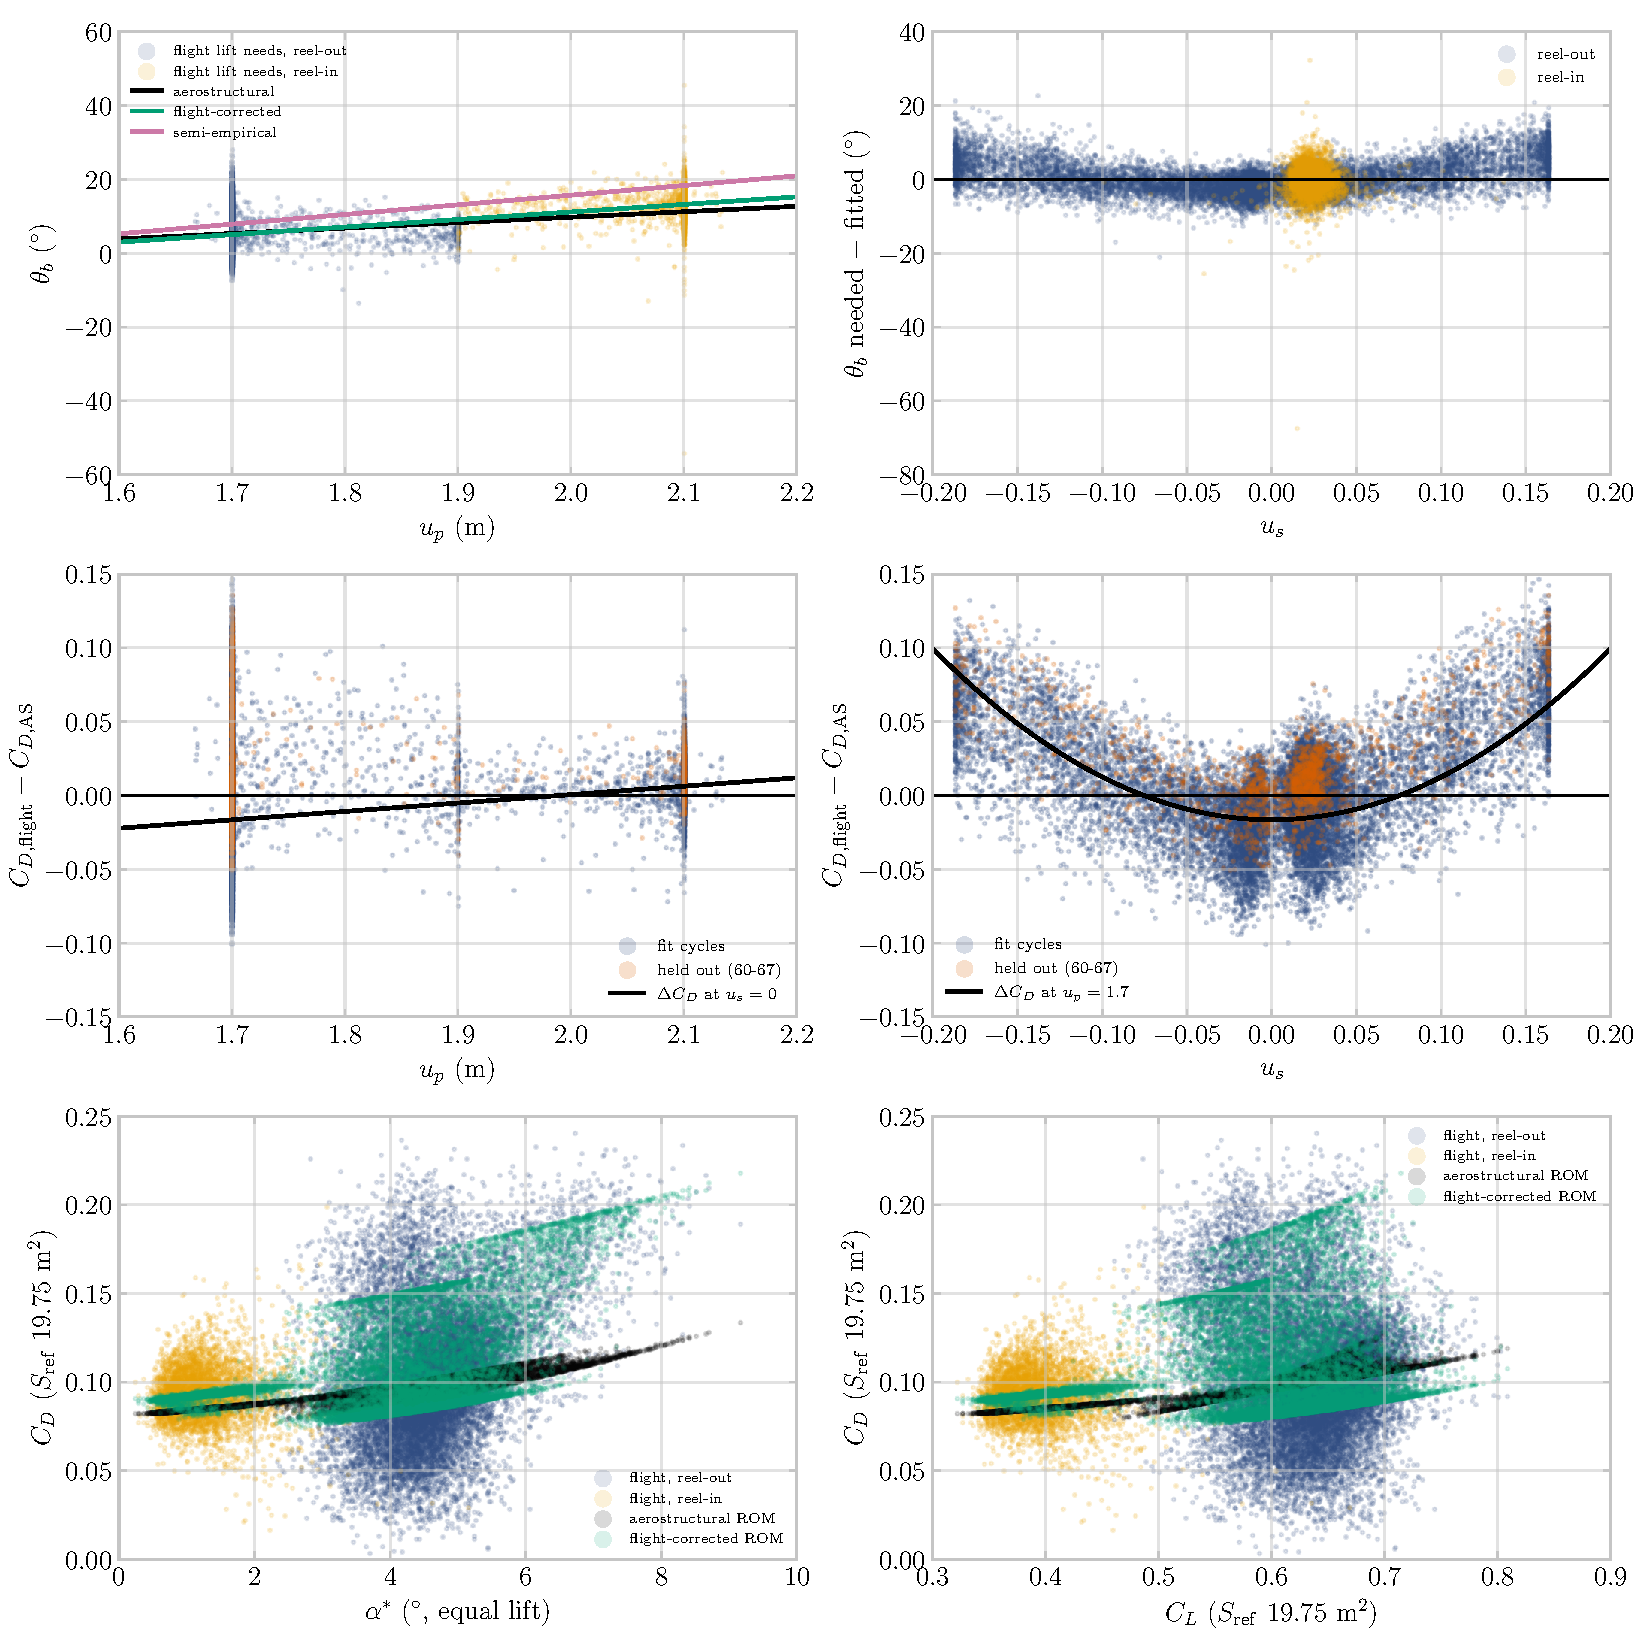
\includegraphics[width=\textwidth]{flight_correction.pdf}
\caption{Steps 1--2 on the 2019 flight. Top: the $\theta_b$ the flight lift
needs against $u_p$, with the aerostructural, flight-corrected (steps 1--2)
and semi-empirical relations, and its residual against steering. Middle: the
drag residual at equal lift against $u_p$ and $u_s$, fit and held-out
cycles. Bottom: drag against $\alpha^*$ and the drag polar.}
\label{fig:fc}
\end{figure}}{}

Two cautions on what these fits mean. The measured roll is almost entirely
the wing's inertia term: in the EKF's own force balance
$\mathbf F_w+\mathbf F_b=m_w(\mathbf a-\mathbf g)$, so the roll of the wing
force relative to the bridle resultant \emph{is} $m_w a_n/|\mathbf F|$, and
it correlates with $u_s$ because steering turns the kite. Without the inertia
term the fitted gain collapses to $-0.09$ ($R^2=0.06$), and it scales with the
wing mass assumed (\SI{11}{\kilogram}: $-0.60$; \SI{17}{\kilogram}: $-0.91$).
It is a turn-response-per-steering times a mass split, not an aerodynamic
measurement on its own, and it is the roll the wing \emph{had} at the turn
it made, against every other normal force the point-mass model puts on the
kite; Sect.~\ref{sec:fc-result} shows it reads \SI{20}{\percent} too strong
once compared with the turn-rate law. It serves as the starting value and as
a check of the sign and order of magnitude. And the equal-lift drag rise with steering
sits where the EKF is least reliable: at $|u_s|>0.12$ its innovation
statistics are 2--3$\times$ worse than in straight flight and the inertial
force is of the order of the drag.

\subsection{Step 3: output error on the quasi-steady solve}
Steps 1--2 match the flight coefficients at the flown states, but the
quasi-steady reconstruction with them still over-predicts the held-out
reel-out ($+19\,\%$ tension, $+12\,\%$ speed). The flown samples are not
equilibria: $|m\dot v_\tau|/D$ is 0.1 at the median and 0.3 at the 90th
percentile on reel-out, and the EKF coefficients are instantaneous, whereas
the ROM is used as a quasi-steady model. Step 3 therefore refits all six
parameters together on the output the ROM is used for: the quasi-steady
ground tension and tangential speed with the measured turn rate in and the
steering solved, on the rigid tether of the optimisations
(\code{refine\_rom\_flight\_output\_error.py}). Tension and speed barely
see the roll gain, which mostly sets how much steering the solve uses, so
the gain gets its own condition, the turn-rate law the paper defines the
steering by: the solved steering must regress 1:1 on the logged steering
(zero offset, \SI{0.3}{\second} lag) over the reel-out training samples, one
residual $5\,(\text{slope}-1)$ with its exact Jacobian from the per-sample
sensitivities. The condition pins the gain only if drag cannot buy
steering: left free, the fit met the slope with the gain at $-0.77$ and the
total $u_s^2$ drag driven to $-0.25$ (a negative steering drag, which makes
the solve fly faster and roll less at high steering), so the steering-drag
coefficients are bounded at zero in total, $C_D$ non-decreasing with
steering. Holding the gain with the measured aerodynamic roll of step 2
instead was tried first and gives $-0.75$; Sect.~\ref{sec:fc-result} shows
why that is \SI{20}{\percent} too strong. \fcSamples{} samples from \fcCycles{} training cycles
enter, half reel-out, half reel-in. Each sample's root is found by Newton's
method, warm-started from its last root, and its derivative with respect to
the parameters follows from the implicit-function theorem, so the outer
Gauss--Newton (trust region) has exact Jacobians. A sample that loses its
root, or whose root lies past the stall, is charged a fixed error instead.
One large NLP with every sample's balance as a constraint was tried first
and is infeasible: reel-in samples sit at the fold of the radial balance
(Sect.~\ref{sec:open}) and lose their root when the parameters move. A
variant that let a steering error (solved against logged $u_s$) hold the
gain instead of the measured roll drove it to a non-physical $-4.9$, the
logged steering explaining the turn poorly (lag; gravity and tether turn
the kite at zero steering), and is not used.

\IfFileExists{generated/flight_correction_params.tex}{%
\begin{table}[H]
\centering\small
\caption{Bridle pitch, drag correction and roll gain. Drag terms are
corrections to the aerostructural $C_D$ (whose own $u_s^2$ coefficient is
about $-0.53$). Steps 1--2 with the cycle-bootstrap 95\,\% interval; step 3 is
the adopted ROM.}
\label{tab:fc-params}
\begin{tabular}{lrrrr}
\toprule
Parameter & Aerostructural & Steps 1--2 (95\,\% CI) & Step 3 & Step 3, reel-out only \\
\midrule
$\theta_0$ (\si{\radian}) & $-0.345$ & $-0.518$ [$-0.543$, $-0.491$] & $-0.587$ & $-0.512$ \\
$\theta_1$ (\si{\radian\per\metre}) & $0.258$ & $0.357$ [$+0.343$, $+0.370$] & $0.41$ & $0.368$ \\
$\Delta C_{D,0}$ & $0$ & $-0.113$ [$-0.130$, $-0.095$] & $-0.182$ & $-0.263$ \\
$\Delta C_{D}$: $u_p$ (\si{\per\metre}) & $0$ & $0.0569$ [$+0.049$, $+0.065$] & $0.103$ & $0.166$ \\
$\Delta C_{D}$: $u_s^2$ & $0$ & $2.9$ [$+2.868$, $+2.929$] & $2.82$ & $0.525$ \\
$k_{\phi,s}$ (\si{\radian}) & $-0.53$ & $-0.765$ [$-0.772$, $-0.758$] & $-0.666$ & $-0.701$ \\
\bottomrule
\end{tabular}

\end{table}}{}

\IfFileExists{generated/flight_correction_training.tex}{%
\begin{table}[H]
\centering\small
\caption{Quasi-steady reconstruction of the \fcCycles{} training cycles
(median errors, steering solved, rigid tether) with the step 1--2 and the
step 3 values; $u_s$ rms against the logged steering plus the zero offset.}
\begin{tabular}{llrrrr}
\toprule
Phase & Parameters & $F_t$ error (\%) & $v_\tau$ error (\%) & $u_s$ rms & Solved (\%) \\
\midrule
reel-out & steps 1--2 & $10.4$ & $4.81$ & $0.036$ & 100 \\
 & step 3 & $-5.98$ & $-4.36$ & $0.039$ & 87 \\
 & step 3, reel-out only & $-2.3$ & $-6.08$ & $0.038$ & 92 \\
reel-in & steps 1--2 & $23.3$ & $6.66$ & $0.012$ & 100 \\
 & step 3 & $17.1$ & $-13.2$ & $0.01$ & 99 \\
\bottomrule
\end{tabular}

\end{table}}{}

\subsection{Result}
\label{sec:fc-result}
\paragraph{The steering gain against the turn-rate law.} The empirical
turn-rate law $\dot\chi = K\,v_a u_s + c_g\,g\cos\beta\sin\chi/v_\tau$
fitted to the 2019 reel-out (logged $u_s$ with the zero offset and the
\SI{0.3}{\second} lag) gives $K=\turnK$\,\si{\radian\per\metre} and
$c_g=\turnG$; a point mass has $c_g=1$, so the kite turns under gravity
about half as much as its mass would, its yaw stiffness resisting course
changes it was not steered into. The same regression on each ROM's turn rate
in the logged-steering mode (Table~\ref{tab:turn-law}) is the check of the
gain: with the gain from the measured roll ($-0.75$) the flight-corrected ROM
gave $K=0.41$, \SI{20}{\percent} above the flight, with the aerostructural
gain ($-0.53$) $K=0.27$; and every ROM has $c_g\approx1.1$--$1.2$, i.e.
2--2.5$\times$ the flight's gravity-driven turn. The two are coupled: the
measured roll is the roll needed to make the measured turn \emph{against}
that exaggerated gravity turn, which is why it over-reads the gain. The
turn-rate-law condition of step 3 sets the gain where the solved steering
regresses 1:1 on the logged one: $-0.67$ for the flight-corrected ROM and
$-0.69$ for the recalibrated semi-empirical one, whose held-out $K$ are
$\turnKaerostructuralflight$ and $\turnKsemiempirical$. The gravity-turn
excess is a property of the point-mass force model (Sect.~\ref{sec:open}).

\IfFileExists{generated/turn_law.tex}{%
\begin{table}[H]
\centering\small
\caption{Turn-rate law fitted to the flight and to each ROM's reconstructed
turn rate (logged steering in, reel-out, cycles 60--67).}
\label{tab:turn-law}
\begin{tabular}{lrrr}
\toprule
$\dot\chi$ of & $K$ (\si{\radian\per\metre}) & $c_g$ & $R^2$ \\
\midrule
flight & 0.343 & 0.47 & 0.875 \\
semi-empirical & 0.383 & 1.22 & 0.889 \\
aerostructural & 0.270 & 1.00 & 0.878 \\
aerostructural-flight & 0.377 & 1.17 & 0.875 \\
\bottomrule
\end{tabular}

\end{table}}{}

\IfFileExists{figures/turn_rate_law.pdf}{%
\begin{figure}[H]
\centering
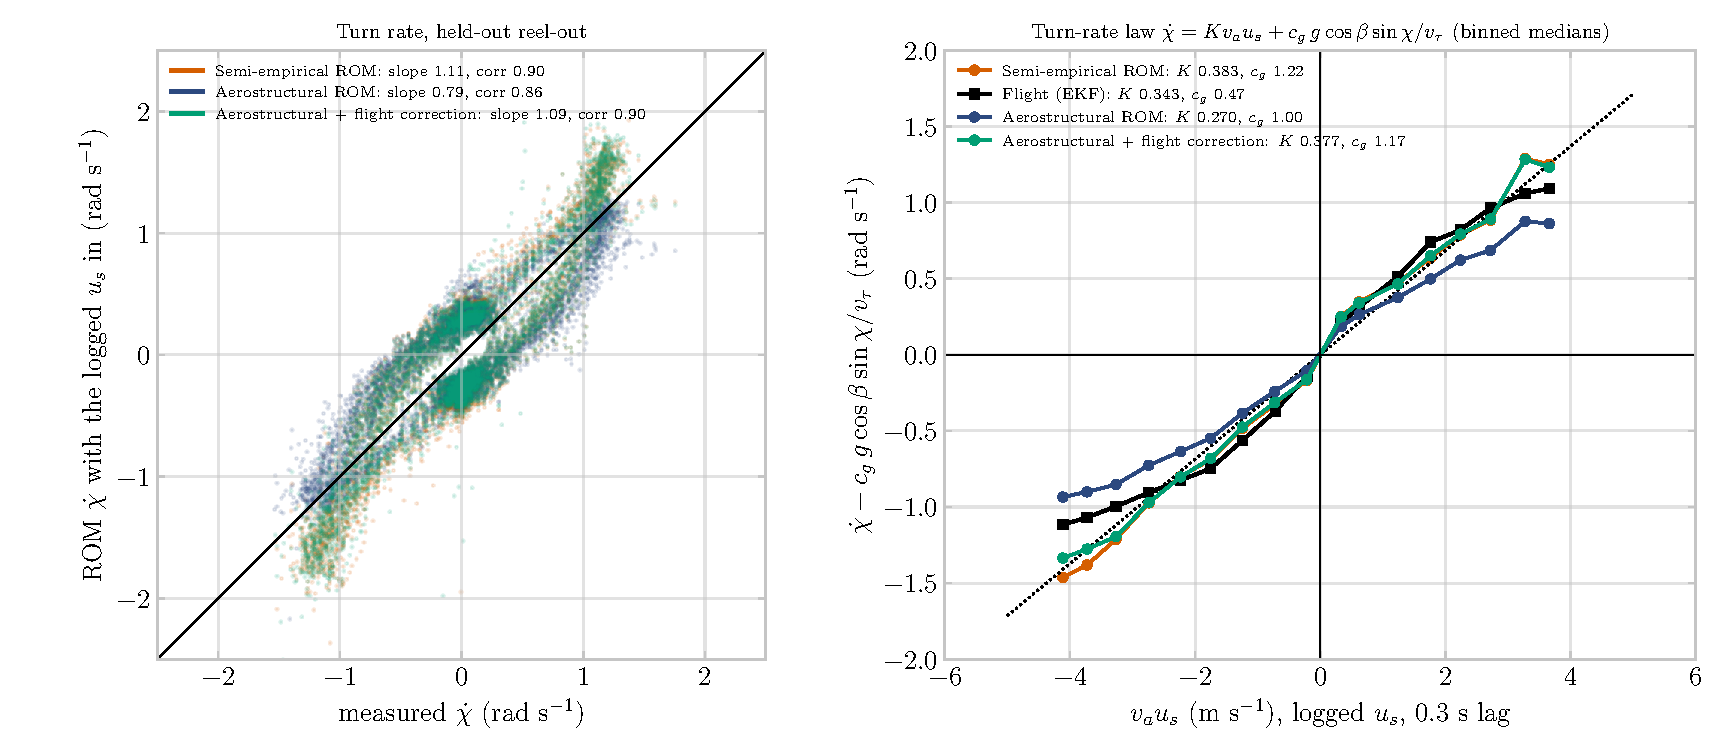
\includegraphics[width=\textwidth]{turn_rate_law.pdf}
\caption{The turn rate of each ROM with the logged steering as input against
the measured one (left, held-out reel-out samples), and the turn-rate law
with the gravity term removed, binned in $v_a u_s$ (right): the flight
against the ROMs. The tuned ROMs sit on the flight's $K$ within
\SI{10}{\percent}; the aerostructural gain under-turns by a third. The
flight's response bends below linear beyond $|v_a u_s|\approx3$, a
saturation at full steering that a linear gain cannot follow, which is where
the tuned ROMs' peak turn rates overshoot.}
\label{fig:turn-law}
\end{figure}}{}

\paragraph{Held out.}
On the held-out cycles (Table~\ref{tab:flight},
Figs.~\ref{fig:flight-solved-64} and~\ref{fig:flight-solved-61}), with the turn
rate in, the corrected ROM reproduces the reel-out tension and speed to
$-3\,\%$ and $-1\,\%$ (median) and the reel-in to $+32\,\%$ and $0\,\%$,
with its solved steering on the logged one (slope 0.88, correlation 0.89).
With the logged steering in, it reproduces the reel-out to $+1\,\%$ and
$+4\,\%$ (semi-empirical: $-6\,\%$ and $-1\,\%$) and the turn rate with
correlation 0.90, and the reel-in tension again to $+33\,\%$; with the
Williams tether the reel-in tension error drops to $+20\,\%$.
\fcValidPct{}\,\% of the training samples keep a valid root at the step-3
parameters. Refitting on the reel-out samples alone (last column of
Table~\ref{tab:fc-params}) moves $\theta_b$ by $0.2^\circ$ at the powered and
$0.7^\circ$ at the depowered setting and the gain by \SI{5}{\percent}: the
reel-out parameters do not depend on the reel-in samples' pull.

Three cautions on the parameters themselves:
\begin{itemize}
  \item \textbf{$\Delta C_{D,0}$ and $c_p$ are nearly interchangeable.} The
        flown $u_p$ takes essentially two values (\SI{1.7}{\metre} and
        \SI{2.1}{\metre}), so only their sum at those two settings is
        identified; the split between them is not.
  \item \textbf{Lift terms without $\alpha$ would not be identifiable
        either.} A lift offset $\Delta C_{L,0}$ or $c_{L,p}u_p$ raises the lift
        at the operating point exactly as a pitch shift $\Delta\theta_0$ or
        $\Delta\theta_1u_p$ does; tension and speed fix the lift and drag at
        the operating point, not the $\alpha$ they occur at, and the only
        independent $\alpha$ measurement, the EKF's bridle vane, sits
        4$^\circ$ from the force-based angle. Where the depower correction
        lives (pitch or polar) is a modelling choice; it matters only where
        $\alpha$ itself matters, the stall margin.
  \item \textbf{Steering drag is not identified.} At equal lift the flight
        drag rises with steering by $c_s\approx+2.9$; the output error on both
        phases keeps $+2.3$ of it, on the reel-out samples alone it goes to
        the bound at zero with the zero-steering drag level rising by $0.03$
        to compensate. Tension and speed cannot tell a steering drag from a
        drag level, so $c_s$ is a range, 0 to about 2.3, tied to the drag
        level, not a value; a $u_s^2$ lift loss, the natural companion term,
        would sit in the same unidentified regime.
\end{itemize}

%======================================================================
\section{Optimisations}
\label{sec:optimisations}
The three ROMs were run through the reel-out downloop optimisation
(\code{downloop\_pattern.py}: one figure-eight at \SI{8}{\metre\per\second}
and \SI{100}{\metre}, logarithmic wind, rigid tether, power-tape length
bounded to 1.6--\SI{2.2}{\metre}, a 3$^\circ$ stall margin on $\alpha$), on
the optimisation hardware of \path{system.yaml} and on the flown 2019
hardware (KCU \SI{22}{\kilogram} with its turbine), all on the corrected
frame. This is an application of the tuned ROMs, not part of their
identification or validation: no optimisation result enters any fitted
parameter, and none of these loops was flown, so nothing here can be checked
against data. The optimiser lets each ROM pick its own loop
(Fig.~\ref{fig:opt-loops}), so the comparison is of what each ROM thinks the
kite can do, not of one path flown with three polars.

\IfFileExists{generated/optimisations.tex}{%
\begin{table}[H]
\centering\small
\caption{Optimised downloop reel-out per ROM: mean power, mean tension, mean
tangential speed and loop time.}
\label{tab:opt}
\resizebox{\textwidth}{!}{\begin{tabular}{llrrrr}
\toprule
System & ROM & $\bar P$ (\si{\kilo\watt}) & $\bar F_t$ (\si{\kilo\newton}) & $\bar v_\tau$ (\si{\metre\per\second}) & $T$ (\si{\second}) \\
\midrule
optimisation hardware (KCU \SI{8.4}{\kilogram}) & semi-empirical & 7.15 & 4.98 & 23.9 & 9.4 \\
 & aerostructural & 10.42 & 6.18 & 27.1 & 12.8 \\
 & aerostructural-flight & 10.78 & 6.30 & 27.7 & 12.3 \\
\midrule
flown 2019 hardware (KCU \SI{22}{\kilogram} + turbine) & semi-empirical & 5.05 & 4.35 & 22.1 & 12.8 \\
 & aerostructural & 5.49 & 4.44 & 23.4 & 19.3 \\
 & aerostructural-flight & 5.90 & 4.62 & 22.9 & 15.5 \\
\bottomrule
\end{tabular}
}
\end{table}}{}

\IfFileExists{figures/optimisation_loops.pdf}{%
\begin{figure}[H]
\centering
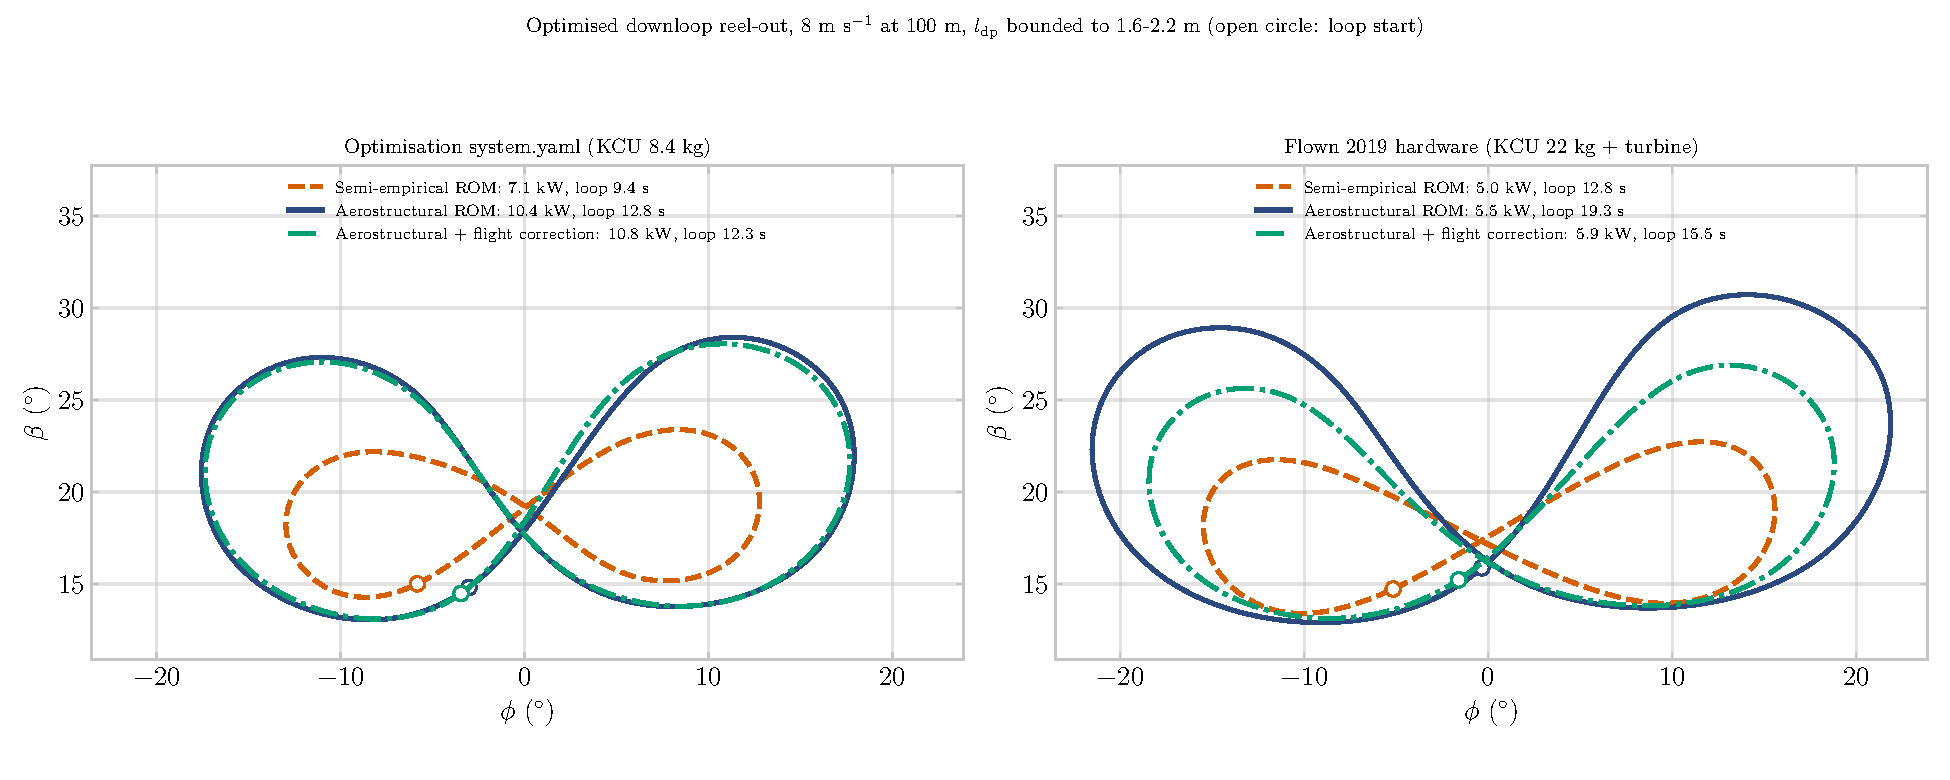
\includegraphics[width=\textwidth]{optimisation_loops.pdf}
\caption{The optimised loops in azimuth and elevation, per ROM and hardware.}
\label{fig:opt-loops}
\end{figure}}{}

On the flown 2019 hardware the three ROMs are within $5.0$--\SI{5.9}{\kilo\watt},
the flight-corrected one highest and the semi-empirical lowest, in the order
of their reel-out tension in the validation. On the lighter optimisation
hardware the two aerostructural ROMs reach \SI{10.4}{\kilo\watt} and
\SI{10.8}{\kilo\watt} against the semi-empirical \SI{7.1}{\kilo\watt}, and fly
taller loops (elevation up to 28$^\circ$ against 23$^\circ$). The difference
is the polar: the aerostructural one has the higher lift-to-drag ratio (it
flew the validation \SI{10}{\percent} faster) and a steering that costs it
little drag, the semi-empirical one carries more drag at the same lift and,
after recalibration, a larger $|u_s|$ drag; with the KCU at
\SI{8.4}{\kilogram} the gravity-driven part of the turn shrinks, and the
higher-$L/D$ polar lets the optimiser pull the loop up and fly it faster.
The spread between the two aerostructural ROMs ($\pm2\,\%$) is
within what the flight correction can resolve; the spread to the
semi-empirical ROM (about a third lower) is a difference of polar shape, not of
calibration, and is not resolved by the 2019 flight, which never flew that
hardware or that pattern.

%======================================================================
\section{Limitations and open points}
\label{sec:open}
\begin{itemize}
  \item \textbf{Reel-in reads as speed-unstable.} At fixed controls, every
        flown 2019 reel-in state reconstructed by the semi-empirical ROM has
        $\partial\dot v_\tau/\partial v_\tau>0$, while reel-out reads
        negative. A $\dot v_\tau(v_\tau)$ sweep at flown states, controls fixed and
        the radial balance solved for the tension at each speed
        (Fig.~\ref{fig:vdot}, \code{sweep\_vdot\_tangential.py}), shows why. On
        reel-out it reproduces the paper's Fig.~6: a stable fast root at the
        reconstructed speed and an unstable post-stall root below it at the
        fastest state; at the slower reel-out states (\SI{12}{\metre\per\second}
        to \SI{15}{\metre\per\second} measured) the branch through the
        reconstructed root already ends at a fold below the measured speed,
        the reconstruction sitting low ($-7\,\%$ in the median,
        Table~\ref{tab:flight}). On reel-in there is no fast root at any
        state. Each branch \emph{ends}, at
        $v_\tau\approx3$--\SI{7}{\metre\per\second}, where no tension can
        balance the radial forces any more: tension also pitches the bridle
        resultant, so the radial residual has a maximum over tension that
        crosses zero at that speed (a fold). The flown reel-in states sit
        within about \SI{1}{\metre\per\second} of the fold, where
        $\partial\dot v_\tau/\partial v_\tau>0$. In this model the kite reels in
        as fast as the radial balance allows. The straight, rigid tether is
        weakest exactly at this low tension, so the sweep was repeated with the
        Williams tether, the radial row solved together with the ground
        closure (Fig.~\ref{fig:vdot-williams}). The fold survives: the reel-in
        branches still end at $v_\tau\approx4$--\SI{7}{\metre\per\second}
        with $\partial\dot v_\tau/\partial v_\tau>0$. The fold is a property
        of the kite model, not of the tether model.
  \item \textbf{Steering range.} The steering terms are identified up to
        $|u_s|\approx0.18$. Beyond it the lift loss with steering
        ($\propto\alpha u_s^2$) extrapolates quadratically, and tight seed
        paths that need more steering are not followable.
  \item \textbf{Stall.} The stall is that of VSM with artificial viscosity on
        frozen deformed shapes; it locates the lift maximum but is the least
        validated part of the model.
  \item \textbf{Centre of the window, gravity off.} Position-dependent
        aerodynamics (sideslip, gravity-induced attitude) are outside the data.
  \item \textbf{Drag deficit.} Most of the apparent deficit was the frame
        error of Sect.~\ref{sec:frame}; what remains ($+7\,\%$ tension,
        $+10\,\%$ speed on reel-out) is within what the flight correction
        absorbs, but it is absorbed by $\theta_b$ and a drag level, which the
        data cannot tell apart from a lift level.
  \item \textbf{Reel-in.} No ROM reproduces both its tension and its speed:
        the aerostructural polar doubles the tension even after the flight
        correction ($+33\,\%$), the recalibrated semi-empirical ROM gets the
        tension ($-7\,\%$) but not the speed ($-18\,\%$). The flown reel-in
        states sit at the fold above, with the kite reeling in near the speed
        the radial balance allows; a quasi-steady point-mass model has one
        knob there, the tension, and the winch transient the kite is actually
        in is outside it.
  \item \textbf{Flight data.} The EKF reconstruction is a model output too:
        its forces depend on its tether model, its coefficients are
        instantaneous at states that are not equilibria, and its innovation
        statistics are 2--3$\times$ worse in turns than in straight flight.
        The cycle bootstrap intervals quoted here cover cycle-to-cycle
        variation only, not these systematic effects, and the 3--4$^\circ$ by
        which the equation-error and output-error $\theta_b$ differ is a
        better measure of what the data pin down.
\end{itemize}

\begin{figure}[H]
\centering
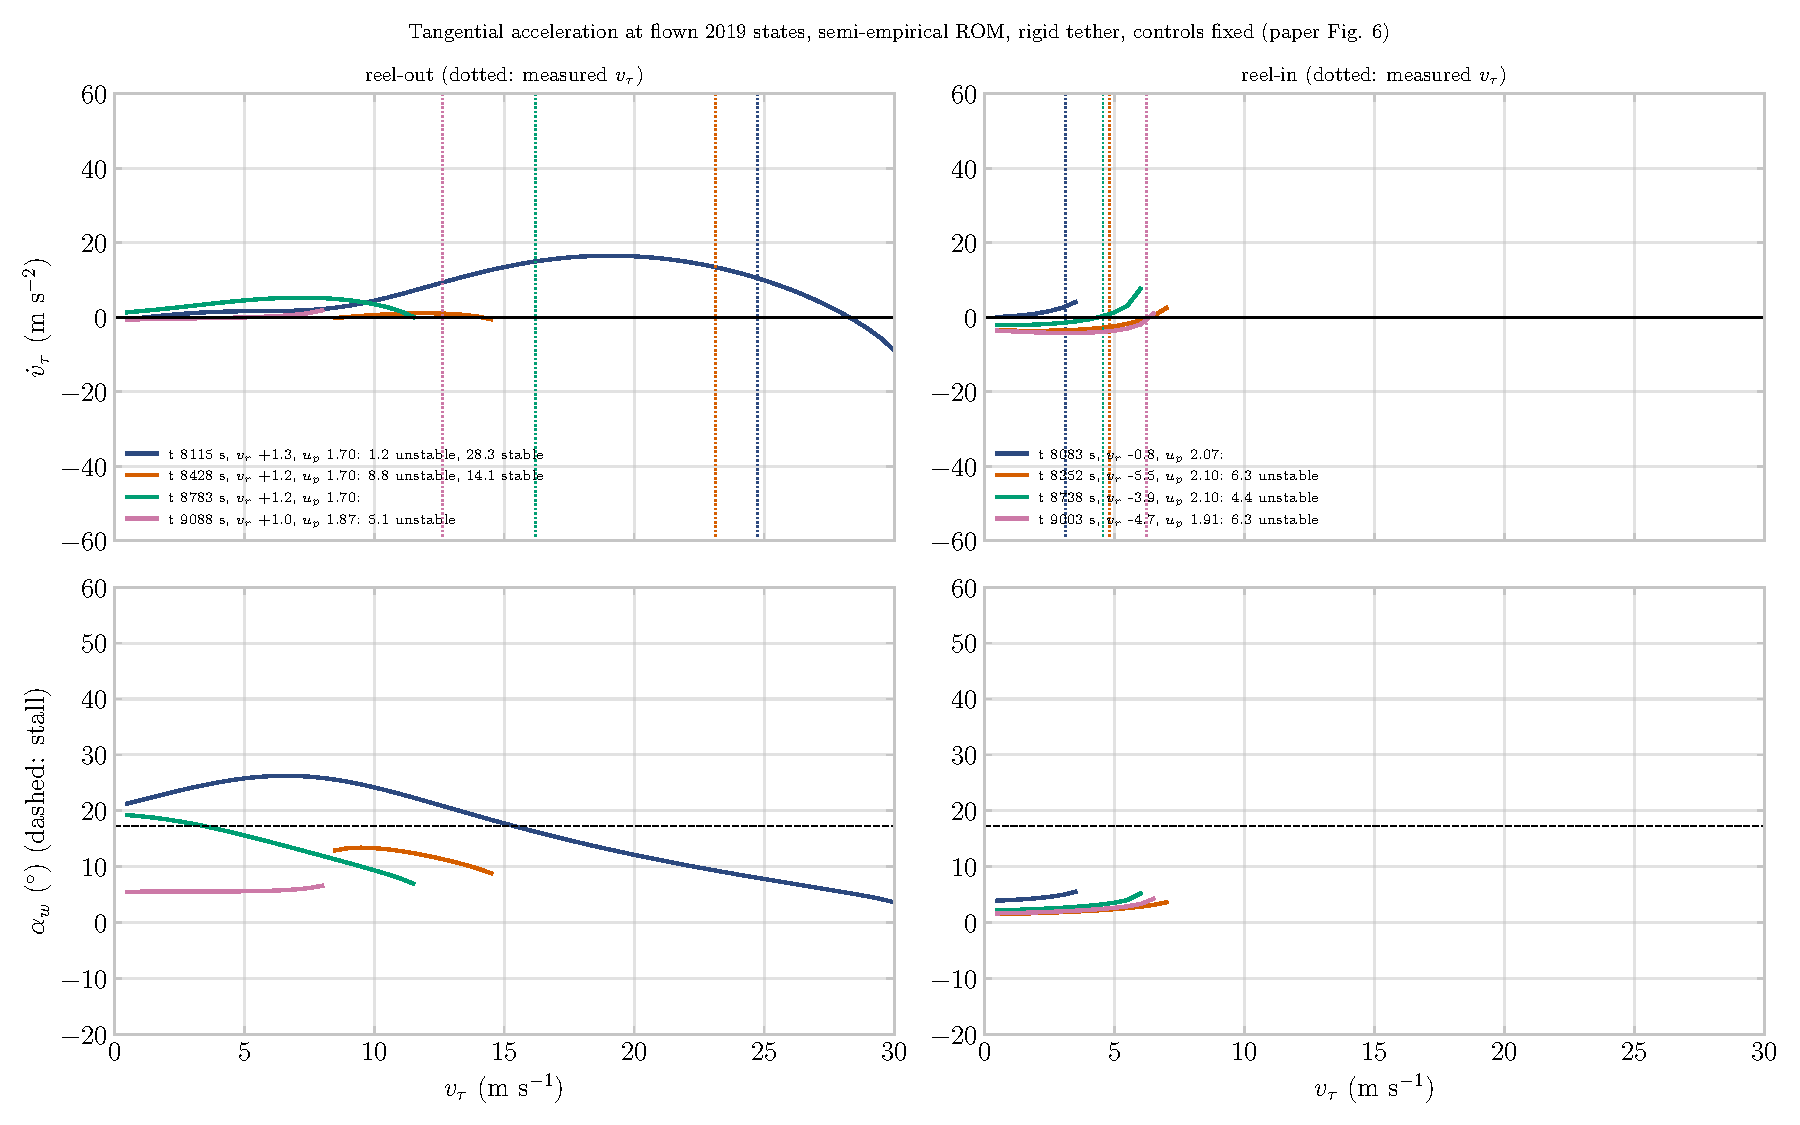
\includegraphics[width=\textwidth]{vdot_sweep.pdf}
\caption{Tangential acceleration and wing angle of attack against tangential
speed at flown 2019 states (semi-empirical ROM, controls fixed, tension from the
radial balance). Reel-in branches end at the fold of the radial balance.}
\label{fig:vdot}
\end{figure}

\IfFileExists{figures/vdot_sweep_williams.pdf}{%
\begin{figure}[H]
\centering
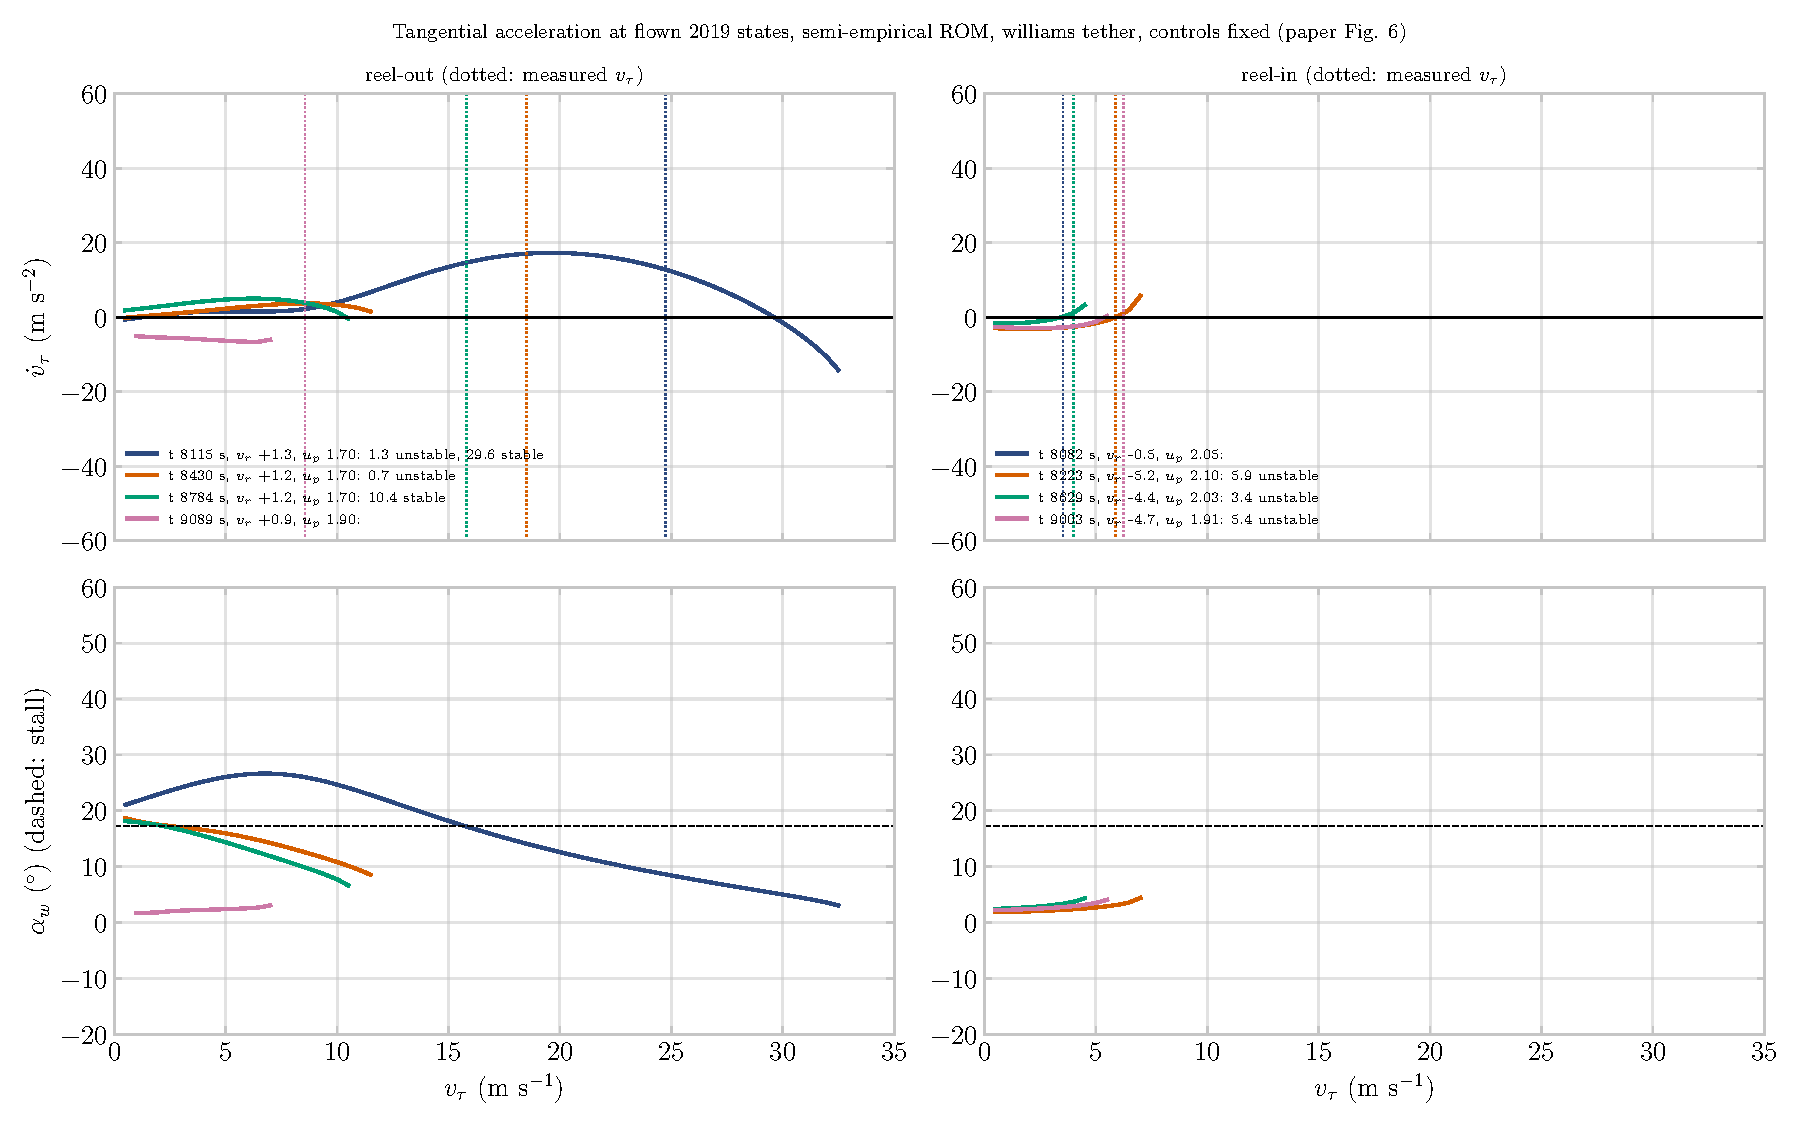
\includegraphics[width=\textwidth]{vdot_sweep_williams.pdf}
\caption{As Fig.~\ref{fig:vdot} with the Williams tether: the radial row and
the ground closure are solved at each speed for the kite-end tension, the
tether length and the last element's angles. The reel-in fold remains.}
\label{fig:vdot-williams}
\end{figure}}{}

%======================================================================
\section{Reproduction}
From the repository root:
\begin{enumerate}
  \item \path{scripts/personal/wes-quasi-steady/run_center_sweep_alpha_polar.py}
        (pinned VSM) for the frozen-shape polars;
  \item \path{scripts/identification/identify_rom_aerostructural.py}, which
        writes the ROM file and the tidy datasets;
  \item \path{scripts/identification/validate_rom_aerostructural.py} and
        \path{plot_rom_comparison.py};
  \item \path{scripts/reduced-order-model/validation/validate_quasi_steady_state_v3.py}
        with \path{--rom <rom> --steering solved|measured}, then
        \path{plot_rom_flight_validation.py};
  \item for the flight correction:
        \path{scripts/identification/identify_rom_flight_correction.py}
        (steps 1--2, writes the ROM file); the validator with
        \path{--rom aerostructural_flight --steering solved --out}
        on training cycles 20--27, 40--47 and 75--82, into
        \path{results/LEI-V3-KITE/identification/rom_flight_correction/output_error/train_*.csv};
        then \path{refine_rom_flight_output_error.py} (step 3, the
        turn-rate-law gain by default, edits the ROM file in place), the
        held-out validation in both modes and
        \path{plot_rom_turn_rate_law.py}; the same with
        \path{--rom semi_empirical} (training CSVs under
        \path{output_error_semi_empirical/}) recalibrates the paper's ROM;
  \item \path{scripts/identification/report_rom_aerostructural.py}, then
        \path{latexmk -pdf} in \path{docs/identification/}.
\end{enumerate}

\begin{thebibliography}{9}
\bibitem{cayon2026rom}
O.~Cayon, V.~van~Deursen and R.~Schmehl,
\emph{Translational dynamics of bridled kites: a reduced-order model in the
course reference frame}, Wind Energ.\ Sci.\ 11, 1097--1121, 2026.

\bibitem{cayon2023vsm}
O.~Cayon, M.~Gaunaa and R.~Schmehl,
\emph{Fast aero-structural model of a leading-edge inflatable kite},
Energies 16, 3061, 2023.

\bibitem{poland2025wind}
J.~A.~W.~Poland, J.~M.~van~Spronsen, M.~Gaunaa and R.~Schmehl,
\emph{Wind tunnel load measurements of a leading-edge inflatable kite rigid
scale model}, Wind Energ.\ Sci.\ Discuss., 2025.
\end{thebibliography}

\end{document}
